%---------------------------------------------------------------------   
    \section{Introducción}
    %------------------------------ SLIDE ---------------------------------------
    \setbeamertemplate{itemize item}{\raisebox{0.2ex}{\scriptsize$\blacktriangleright$}}
    \setbeamercolor{itemize item}{fg=red} % Cambia el color del triángulo a naranja    
    \begin{frame}{Introducción} % cada entorno frame es una diapositiva
        \justifying % para justificar el texto, siempre al inicio de cada frame
        % Añade espacio para mover el bloque hacia arriba
        % Añade espacio para mover el bloque hacia arriba
        \vspace*{-0.6cm} % Ajusta este valor según sea necesario
        
        % Define los colores del bloque
        %\definecolor{custombgcolor2}{RGB}{201, 123, 219} % Color de fondo
        %\definecolor{customfgcolor2}{RGB}{0, 0, 0} % Color del texto

        % Cuadro sin bordes redondeados, con colores personalizados
        \begin{tcolorbox}[colback=custombgcolor2, coltext=customfgcolor2,
                      colframe=custombgcolor2, % Color del borde
                      width=\textwidth,       % Ancho del cuadro
                      boxrule=1pt,            % Grosor del borde
                      top=1mm, bottom=1mm,     % Espacio superior e inferior
                      sharp corners=all,     % Bordes sin redondear
                      halign=center,         % Alineación horizontal
                      valign=center,         % Alineación vertical
                      ]
            % Texto dentro del cuadro
            % \textbf{Rayos \kern-0.9em Cósmicos \kern-0.9em (RC)}
            \textbf{¿Qué \kern-0.9em son \kern-0.9em los \kern-0.9em Rayos \kern-0.9em Cósmicos?}
        \end{tcolorbox}

        \begin{columns}
            \begin{column}{0.7\textwidth} % Columna izquierda para la lista
                \begin{itemize}
                    \item Núcleos de átomos desprovistos de sus electrones. 
                    \item Consisten en $\sim 90\%$ protones, $\sim 9\%$ núcleos de helio y $\sim 1\%$ otros núcleos más pesados.
                    \item Llegan a la Tierra desde todas direcciones.
                    \item Descubiertos por \emph{Victor Hess} en 1912.
                \end{itemize}
            \end{column}

            \begin{column}{0.3\textwidth} % Columna derecha para la imagen
                \begin{figure}
                    \centering
                    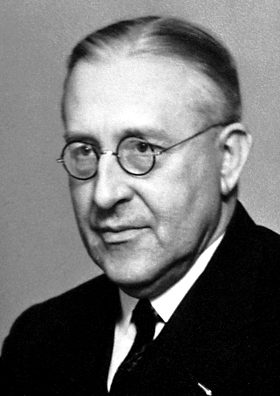
\includegraphics[width=0.6\textwidth]{Figures/vhess.jpg}
                    \caption{\tiny Victor Hess recibió el premio Nobel de Física en 1936 por su descubrimiento de los rayos cósmicos.}
                \end{figure}
            \end{column}            
        \end{columns} 
    \end{frame}

    %------------------------------ SLIDE --------------------------------------- SLIDE DE PRUEBA ESPECTRO DE ENERGIA + METODOS DE DETECCION
    \begin{frame}{} % cada entorno frame es una diapositiva
        \justifying % para justificar el texto, siempre al inicio de cada frame
        % Añade espacio para mover el bloque hacia arriba
        % Añade espacio para mover el bloque hacia arriba
        \vspace*{-0.31cm} % Ajusta este valor según sea necesario
        
        % Define los colores del bloque
        %\definecolor{custombgcolor3}{RGB}{231, 185, 104} % Color de fondo
        %\definecolor{customfgcolor2}{RGB}{0, 0, 0} % Color del texto

        % Cuadro sin bordes redondeados, con colores personalizados
        %\begin{tcolorbox}[colback=custombgcolor3, coltext=customfgcolor2,
                      %colframe=custombgcolor3, % Color del borde
                      %width=\textwidth,       % Ancho del cuadro
                      %boxrule=1pt,            % Grosor del borde
                      %top=1mm, bottom=1mm,     % Espacio superior e inferior
                      %sharp corners=all,     % Bordes sin redondear
                      %halign=center,         % Alineación horizontal
                      %valign=center,         % Alineación vertical
                      %]
            % Texto dentro del cuadro
            %\textbf{Espectro \kern-0.9em de \kern-0.9em Energía}
        %\end{tcolorbox}

        \begin{columns}
            \begin{column}{0.4\textwidth} % Columna izquierda para la lista
                \textcolor{blue}{\textbf{Espectro de energía:}}
                \begin{itemize}
                    \item Ley de potencia: $\bm{\Phi}\mathbf{(E) \propto E}^{\bm{-\alpha}}$,
                    
                    donde $\mathbf{E}$ es la energía y $\bm{\alpha}$ el índice espectral.
                    \item Abarca varios ordenes de magnitud ($\sim \bm{10^{8}}$ a $\sim \bm{10^{21}}$) \textbf{eV}.
                    \item Son muy abundantes los rayos cósmicos de \textbf{baja energía}.
                    \item Los rayos cósmicos pueden ser detectados de manera \textbf{directa} e \textbf{indirecta}.
                    %\item Índice espectral $\bm{\alpha}$.
                    %\item La \textbf{rodilla} es donde se produce un cambio en el valor de $\bm{\alpha}$.
                    %\item En la región del \textbf{tobillo} el valor del índice cambia $\bm{\alpha} \mathbf{\sim 2}$.\textbf{6}.
                \end{itemize}
            \end{column}

            \begin{column}{0.5\textwidth} % Columna derecha para la imagen
                \begin{figure}
                    \centering
                    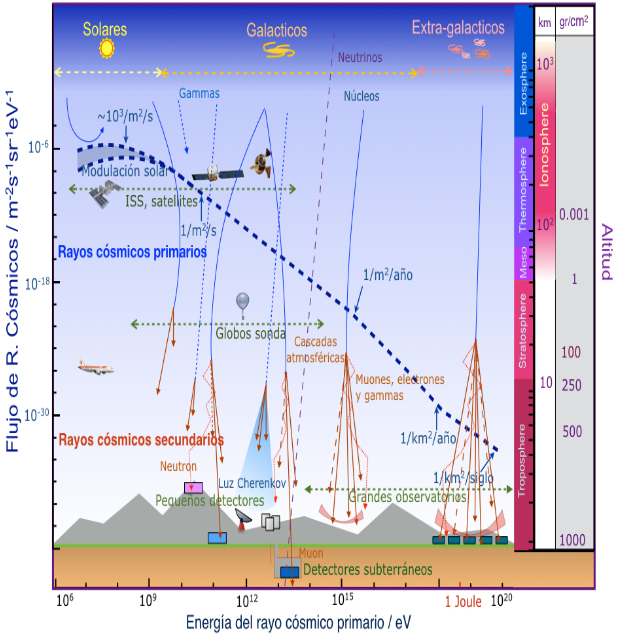
\includegraphics[width=1.0\textwidth]{Figures/spectrum2.png}
                    \caption{\tiny Espectro de los RC, se muestra los instrumentos usados para la detección a diferentes altitudes. Imagen tomada del \href{https://revista.iaa.csic.es/content/portada/404/69}{Instituto de Astrofísica de Andalucía (IAA-CSIC)} (2023).}                    
                \end{figure}
            \end{column}
        \end{columns}
    \end{frame}

    %------------------------------ SLIDE --------------------------------------- SLIDE ORIGINAL ESPECTRO DE ENERGIA
    %\begin{frame}{} % cada entorno frame es una diapositiva
        %\justifying % para justificar el texto, siempre al inicio de cada frame
        % Añade espacio para mover el bloque hacia arriba
        % Añade espacio para mover el bloque hacia arriba
        %\vspace*{-1.55cm} % Ajusta este valor según sea necesario
        
        % Define los colores del bloque
        %\definecolor{custombgcolor3}{RGB}{231, 185, 104} % Color de fondo
        %\definecolor{customfgcolor2}{RGB}{0, 0, 0} % Color del texto

        % Cuadro sin bordes redondeados, con colores personalizados
        %\begin{tcolorbox}[colback=custombgcolor3, coltext=customfgcolor2,
                      %colframe=custombgcolor3, % Color del borde
                      %width=\textwidth,       % Ancho del cuadro
                      %boxrule=1pt,            % Grosor del borde
                      %top=1mm, bottom=1mm,     % Espacio superior e inferior
                      %sharp corners=all,     % Bordes sin redondear
                      %halign=center,         % Alineación horizontal
                      %valign=center,         % Alineación vertical
                      %]
            % Texto dentro del cuadro
            %\textbf{Espectro \kern-0.9em de \kern-0.9em Energía}
        %\end{tcolorbox}

        %\begin{columns}
            %\begin{column}{0.45\textwidth} % Columna izquierda para la lista
                %\begin{itemize}
                    %\item Ley de potencia: $\bm{\Phi}\mathbf{(E) \propto E}^{\bm{-\alpha}}$.
                    %\item La región donde el índice espectral $\bm{\alpha} \mathbf{\sim 2}$.\textbf{7} podrían provenir de nuestra galaxia.
                    %\item La \textbf{rodilla} es donde se produce un cambio en el valor de $\bm{\alpha}$.
                    %\item En la región del \textbf{tobillo} el valor del índice cambia $\bm{\alpha} \mathbf{\sim 2}$.\textbf{6}.
                %\end{itemize}
            %\end{column}

            %\begin{column}{0.4\textwidth} % Columna derecha para la imagen
                %\begin{figure}
                    %\centering
                    %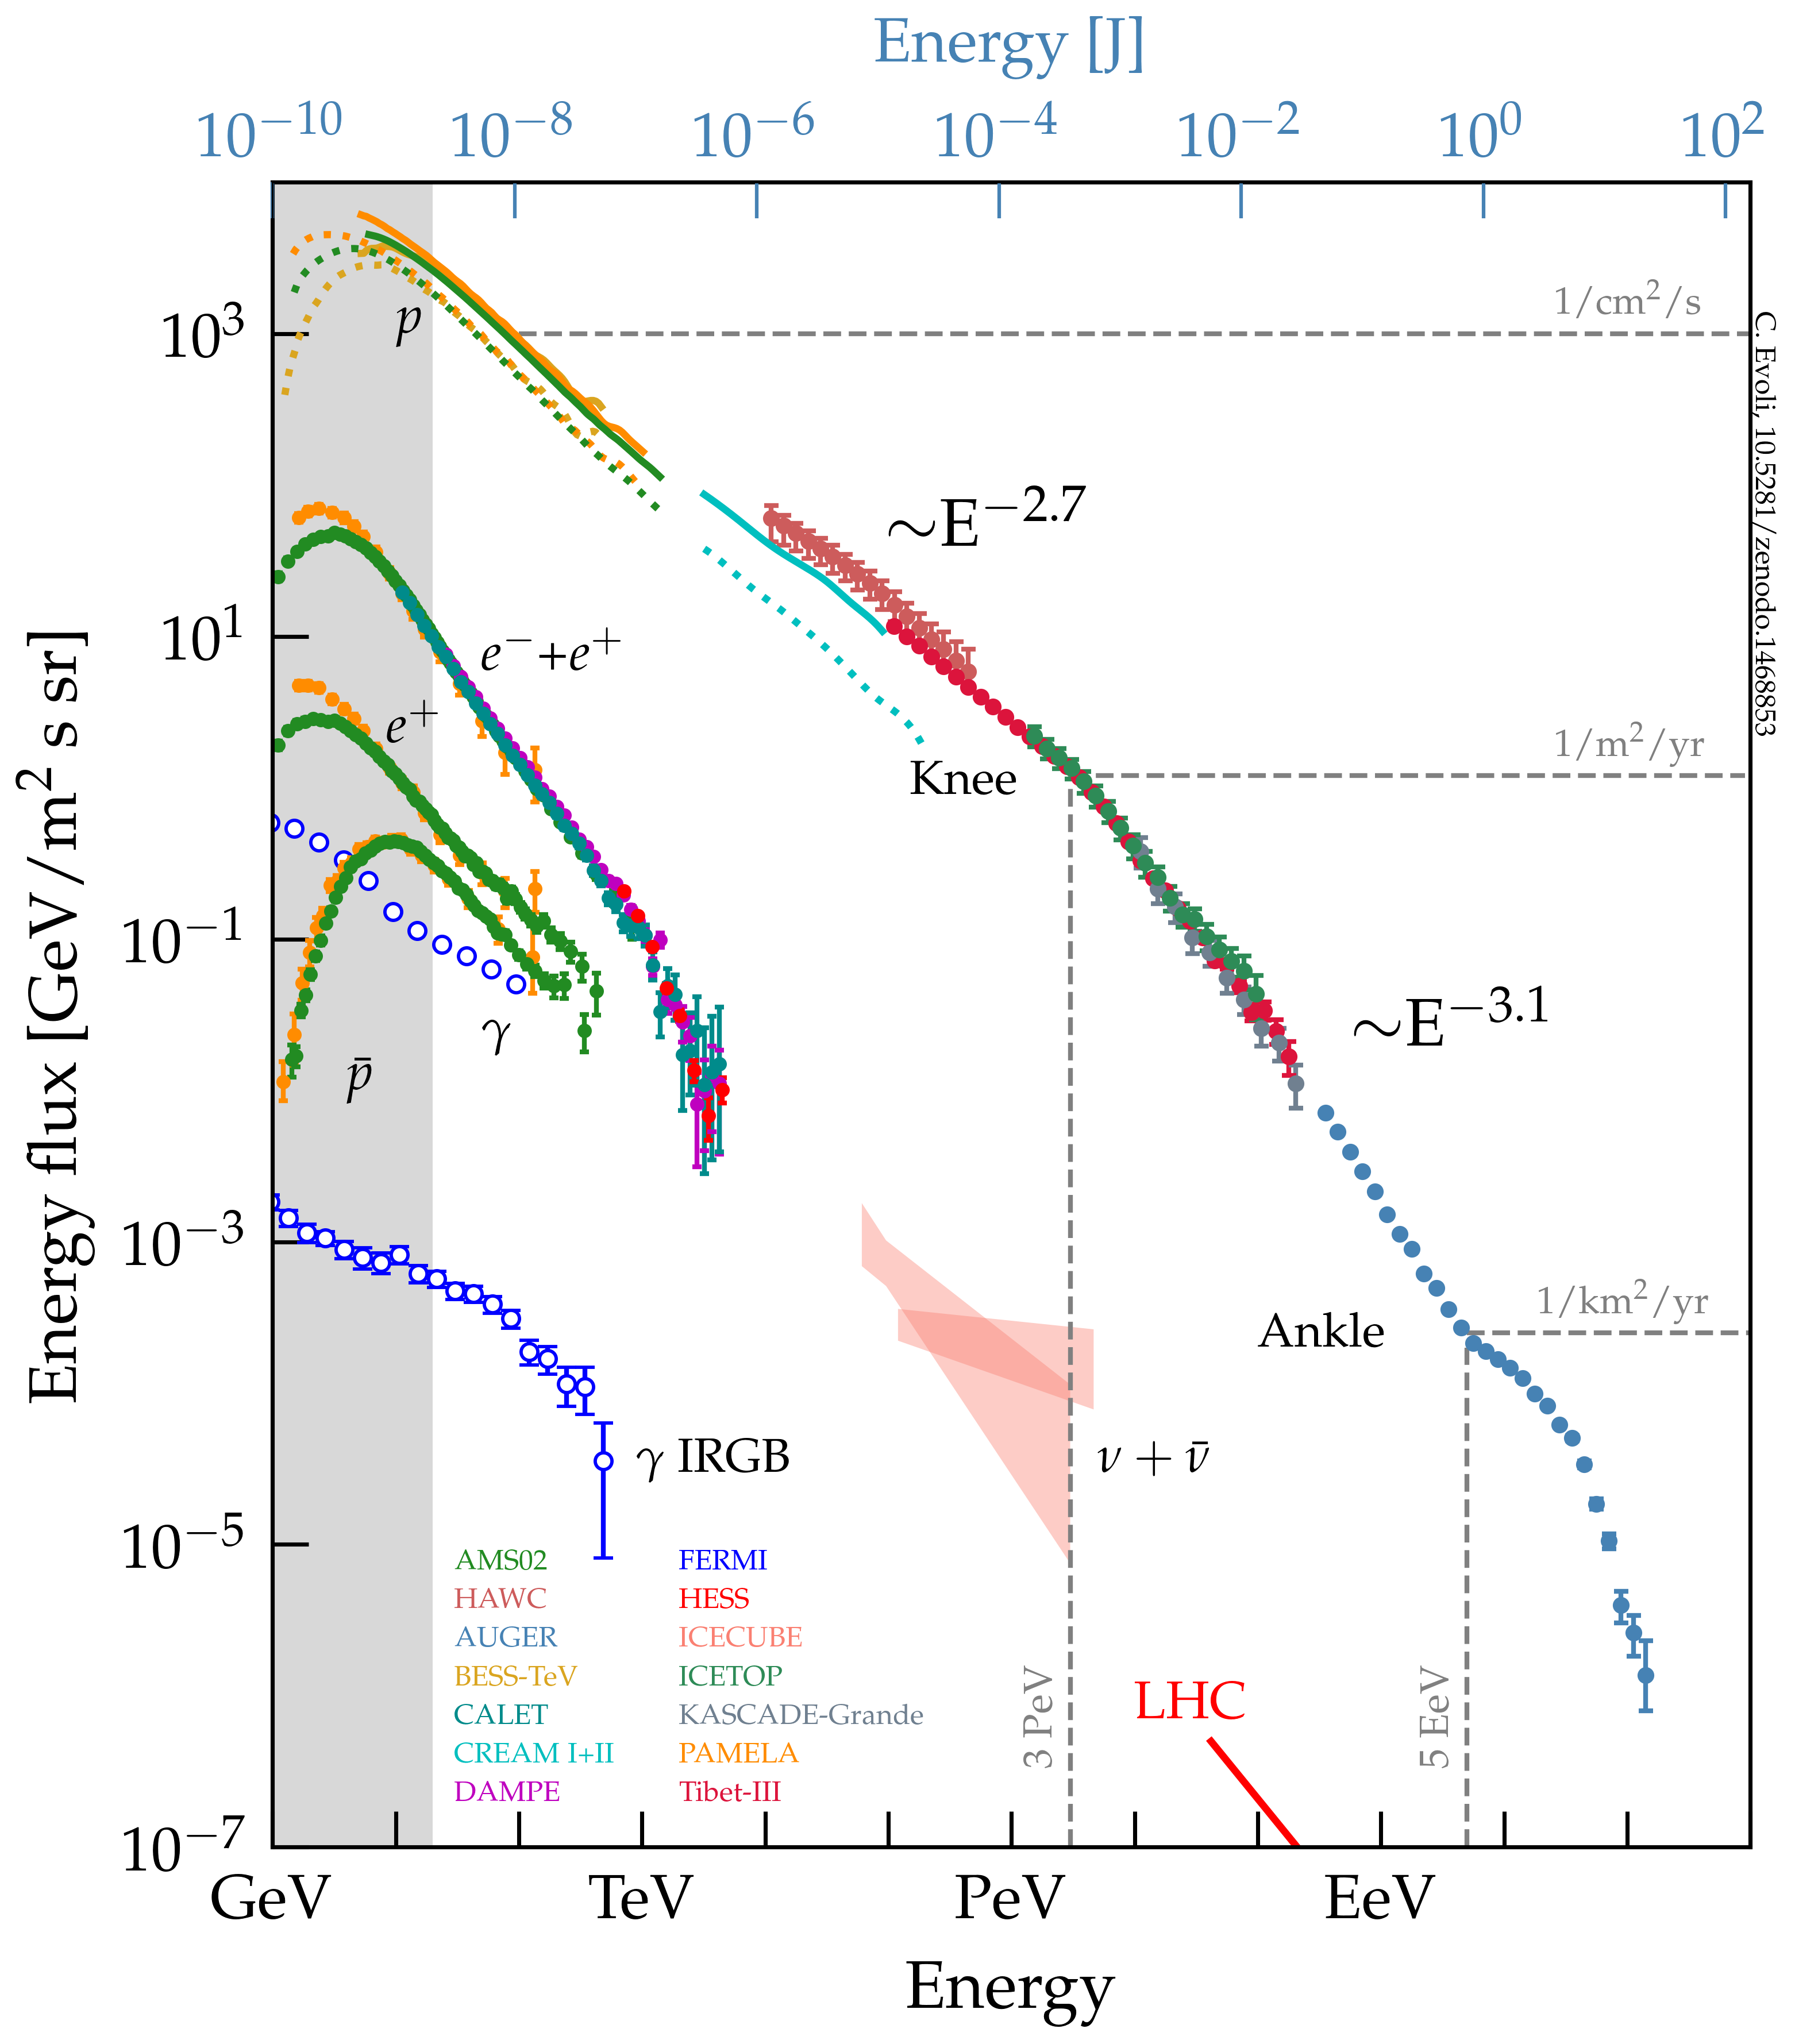
\includegraphics[width=1.0\textwidth]{Figures/spectrum.png}
                    %\caption{\tiny Espectro de energía de los RC [\cite{evoli2018}].}                    
                %\end{figure}
            %\end{column}
        %\end{columns}
    %\end{frame}
    
    %------------------------------ SLIDE --------------------------------------- SLIDE ORIGINAL DE ORIGEN DE RC
    %\begin{frame}{} % cada entorno frame es una diapositiva
        %\justifying % para justificar el texto, siempre al inicio de cada frame
        % Añade espacio para mover el bloque hacia arriba
        % Añade espacio para mover el bloque hacia arriba
        %\vspace*{-0.4cm} % Ajusta este valor según sea necesario

        % Cuadro sin bordes redondeados, con colores personalizados
        %\begin{tcolorbox}[colback=custombgcolor2, coltext=customfgcolor2,
                      %colframe=custombgcolor2, % Color del borde
                      %width=\textwidth,       % Ancho del cuadro
                      %boxrule=1pt,            % Grosor del borde
                      %top=1mm, bottom=1mm,     % Espacio superior e inferior
                      %sharp corners=all,     % Bordes sin redondear
                      %halign=center,         % Alineación horizontal
                      %valign=center,         % Alineación vertical
                      %]
            % Texto dentro del cuadro
            %\textbf{Origen \kern-0.9em de \kern-0.9em los \kern-0.9em Rayos \kern-0.9em Cósmicos}
        %\end{tcolorbox}
        
        %\begin{figure}
        	%\centering
        	%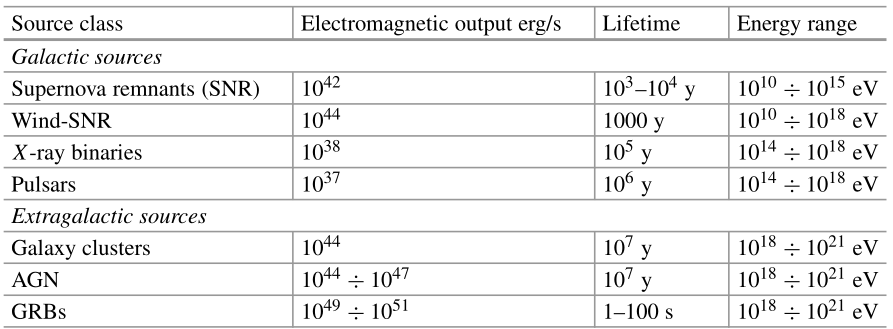
\includegraphics[width=0.5\textwidth]{Figures/sourcestable1.png}
        	%\caption{\tiny Posibles fuentes de rayos cósmicos [\cite{spurio2018}].} 
        %\end{figure}
    %\end{frame}  

    %------------------------------ SLIDE --------------------------------------- SLIDE DE PRUEBA DE ORIGEN DE RC
    \begin{frame}{} % cada entorno frame es una diapositiva
        \justifying % para justificar el texto, siempre al inicio de cada frame
        % Añade espacio para mover el bloque hacia arriba
        % Añade espacio para mover el bloque hacia arriba
        \vspace*{-0.3cm} % Ajusta este valor según sea necesario
        % Cuadro sin bordes redondeados, con colores personalizados
        \begin{tcolorbox}[colback=custombgcolor2, coltext=customfgcolor2,
                      colframe=custombgcolor2, % Color del borde
                      width=\textwidth,       % Ancho del cuadro
                      boxrule=1pt,            % Grosor del borde
                      top=0.1mm, bottom=0.1mm,     % Espacio superior e inferior
                      sharp corners=all,     % Bordes sin redondear
                      halign=center,         % Alineación horizontal
                      valign=center,         % Alineación vertical
                      ]
            % Texto dentro del cuadro
            \textbf{Origen \kern-0.9em de \kern-0.9em los \kern-0.9em Rayos \kern-0.9em Cósmicos}
        \end{tcolorbox}

        \vspace*{0.1cm} % Ajusta este valor según sea necesario
        
        \begin{columns}
            \begin{column}{0.5\textwidth}
                \centering
                \fcolorbox{black}{custombgcolor5}{
                    \parbox[c][0.5cm][c]{0.8\textwidth}{
                        \centering
                        Galáctico
                    }
                }

                \vspace*{0.3cm} % Ajusta este valor según sea necesario
                \begin{figure}
                    \centering
				    \includegraphics[width=1.0\textwidth]{Figures/remanetsupernova1.jpg}
				    \caption{\tiny Remanente de supernova en la \textbf{nebulosa del Cangrejo}, se encuentra a $6500$ años luz de la Tierra. Créditos: Rayos X: NASA/CXC/SAO; Visible: NASA/STScI; Infrarrojo: NASA-JPL-Caltech.}
                \end{figure}
                
            \end{column}

            \begin{column}{0.5\textwidth}
                \centering
                \fcolorbox{black}{custombgcolor7}{
                    \parbox[c][0.5cm][c]{0.8\textwidth}{
                        \centering
                        Extragaláctico
                    }
                }

                \vspace*{0.3cm} % Ajusta este valor según sea necesario
                \begin{figure}
                    \centering
				    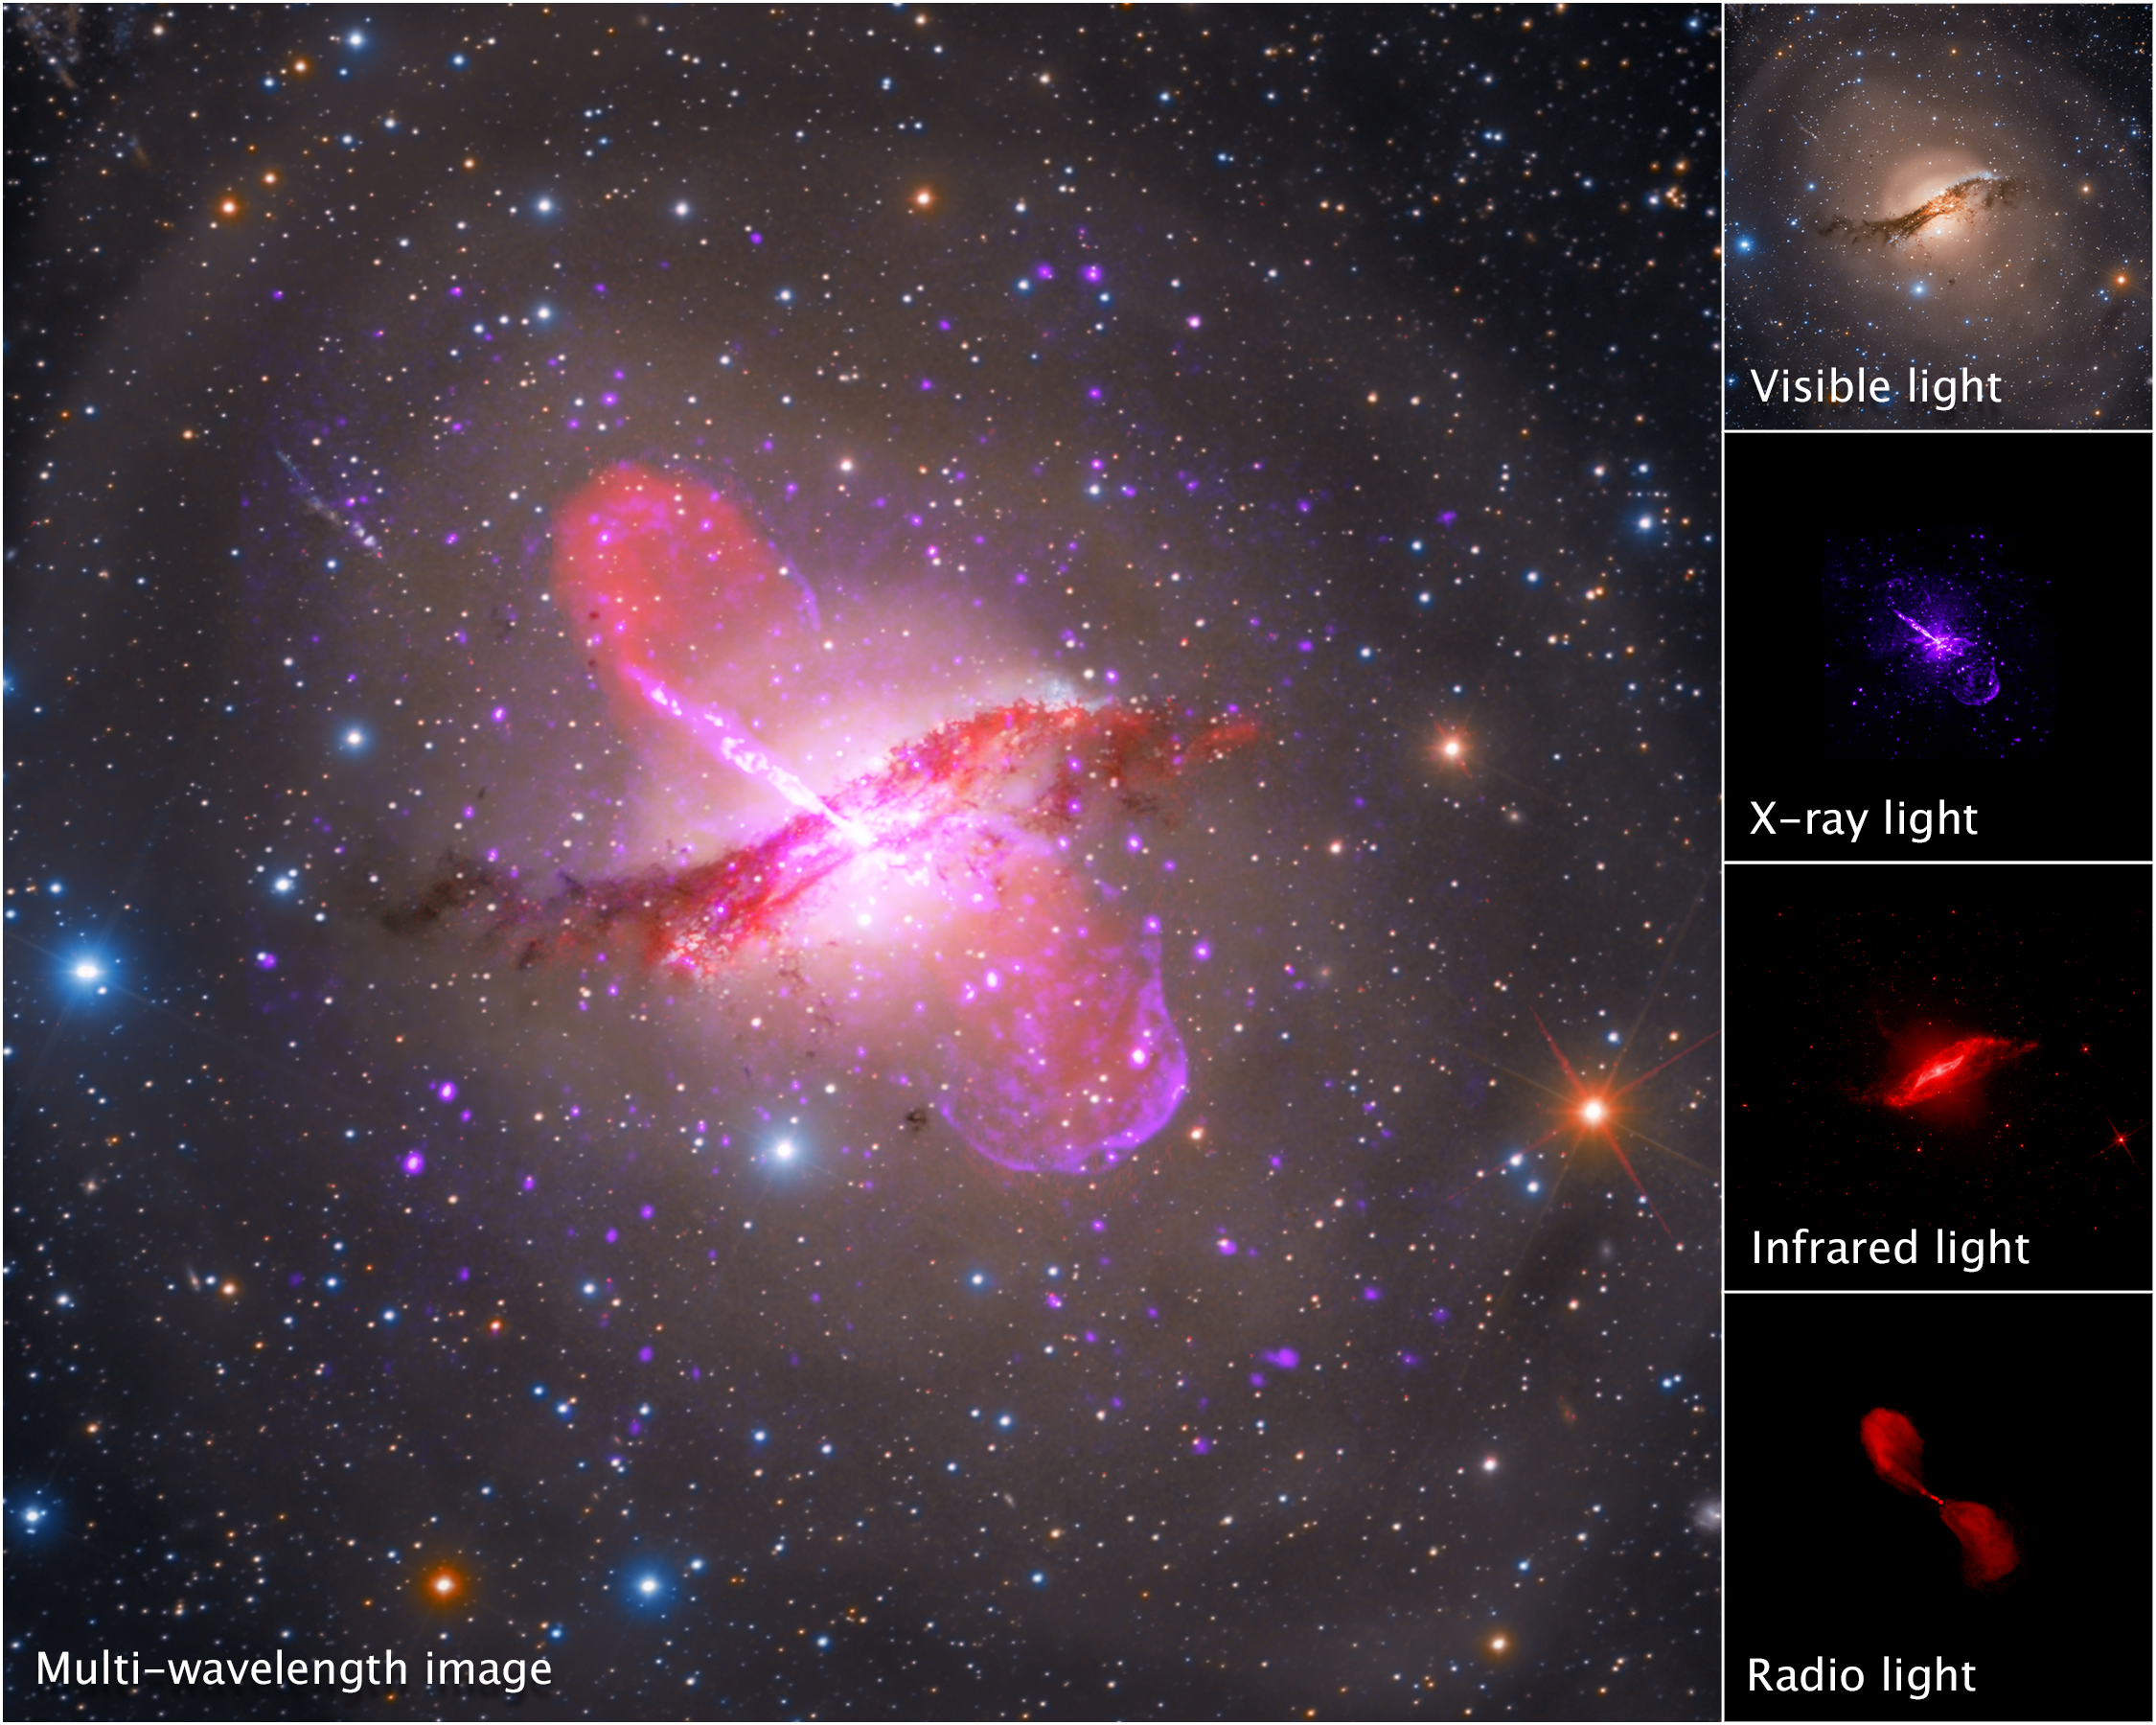
\includegraphics[width=0.8\textwidth]{Figures/centaurusA_multiwavelength.png}
				    \caption{\tiny \textbf{Centaurus A} es una galaxia activa cercana a la Vía Láctea, ubicada a 3.5 megapársecs. Créditos: X-ray: NASA/CXC/SAO; optical: Rolf Olsen; infrared: NASA/JPL-Caltech; radio: NRAO/AUI/NSF/Univ.Hertfordshire/M.Hardcastle.}
                \end{figure}            
            \end{column}
        \end{columns}
    \end{frame}  

	%------------------------------ SLIDE --------------------------------------- SLIDE ORIGINAL DE ORIGEN DE RC
	%\begin{frame}{}
		%\begin{figure}
			%\centering
    		%\begin{minipage}{0.49\textwidth}
				%\includegraphics[width=\textwidth]{Figures/remanetsupernova1.jpg}
				%\caption{\tiny Remanente de supernova en la \textbf{nebulosa del Cangrejo}, se encuentra a $6500$ años luz de la Tierra. Créditos: Rayos X: NASA/CXC/SAO; Visible: NASA/STScI; Infrarrojo: NASA-JPL-Caltech.}
			%\end{minipage}
			%\hfill
			%\begin{minipage}{0.5\textwidth}
				%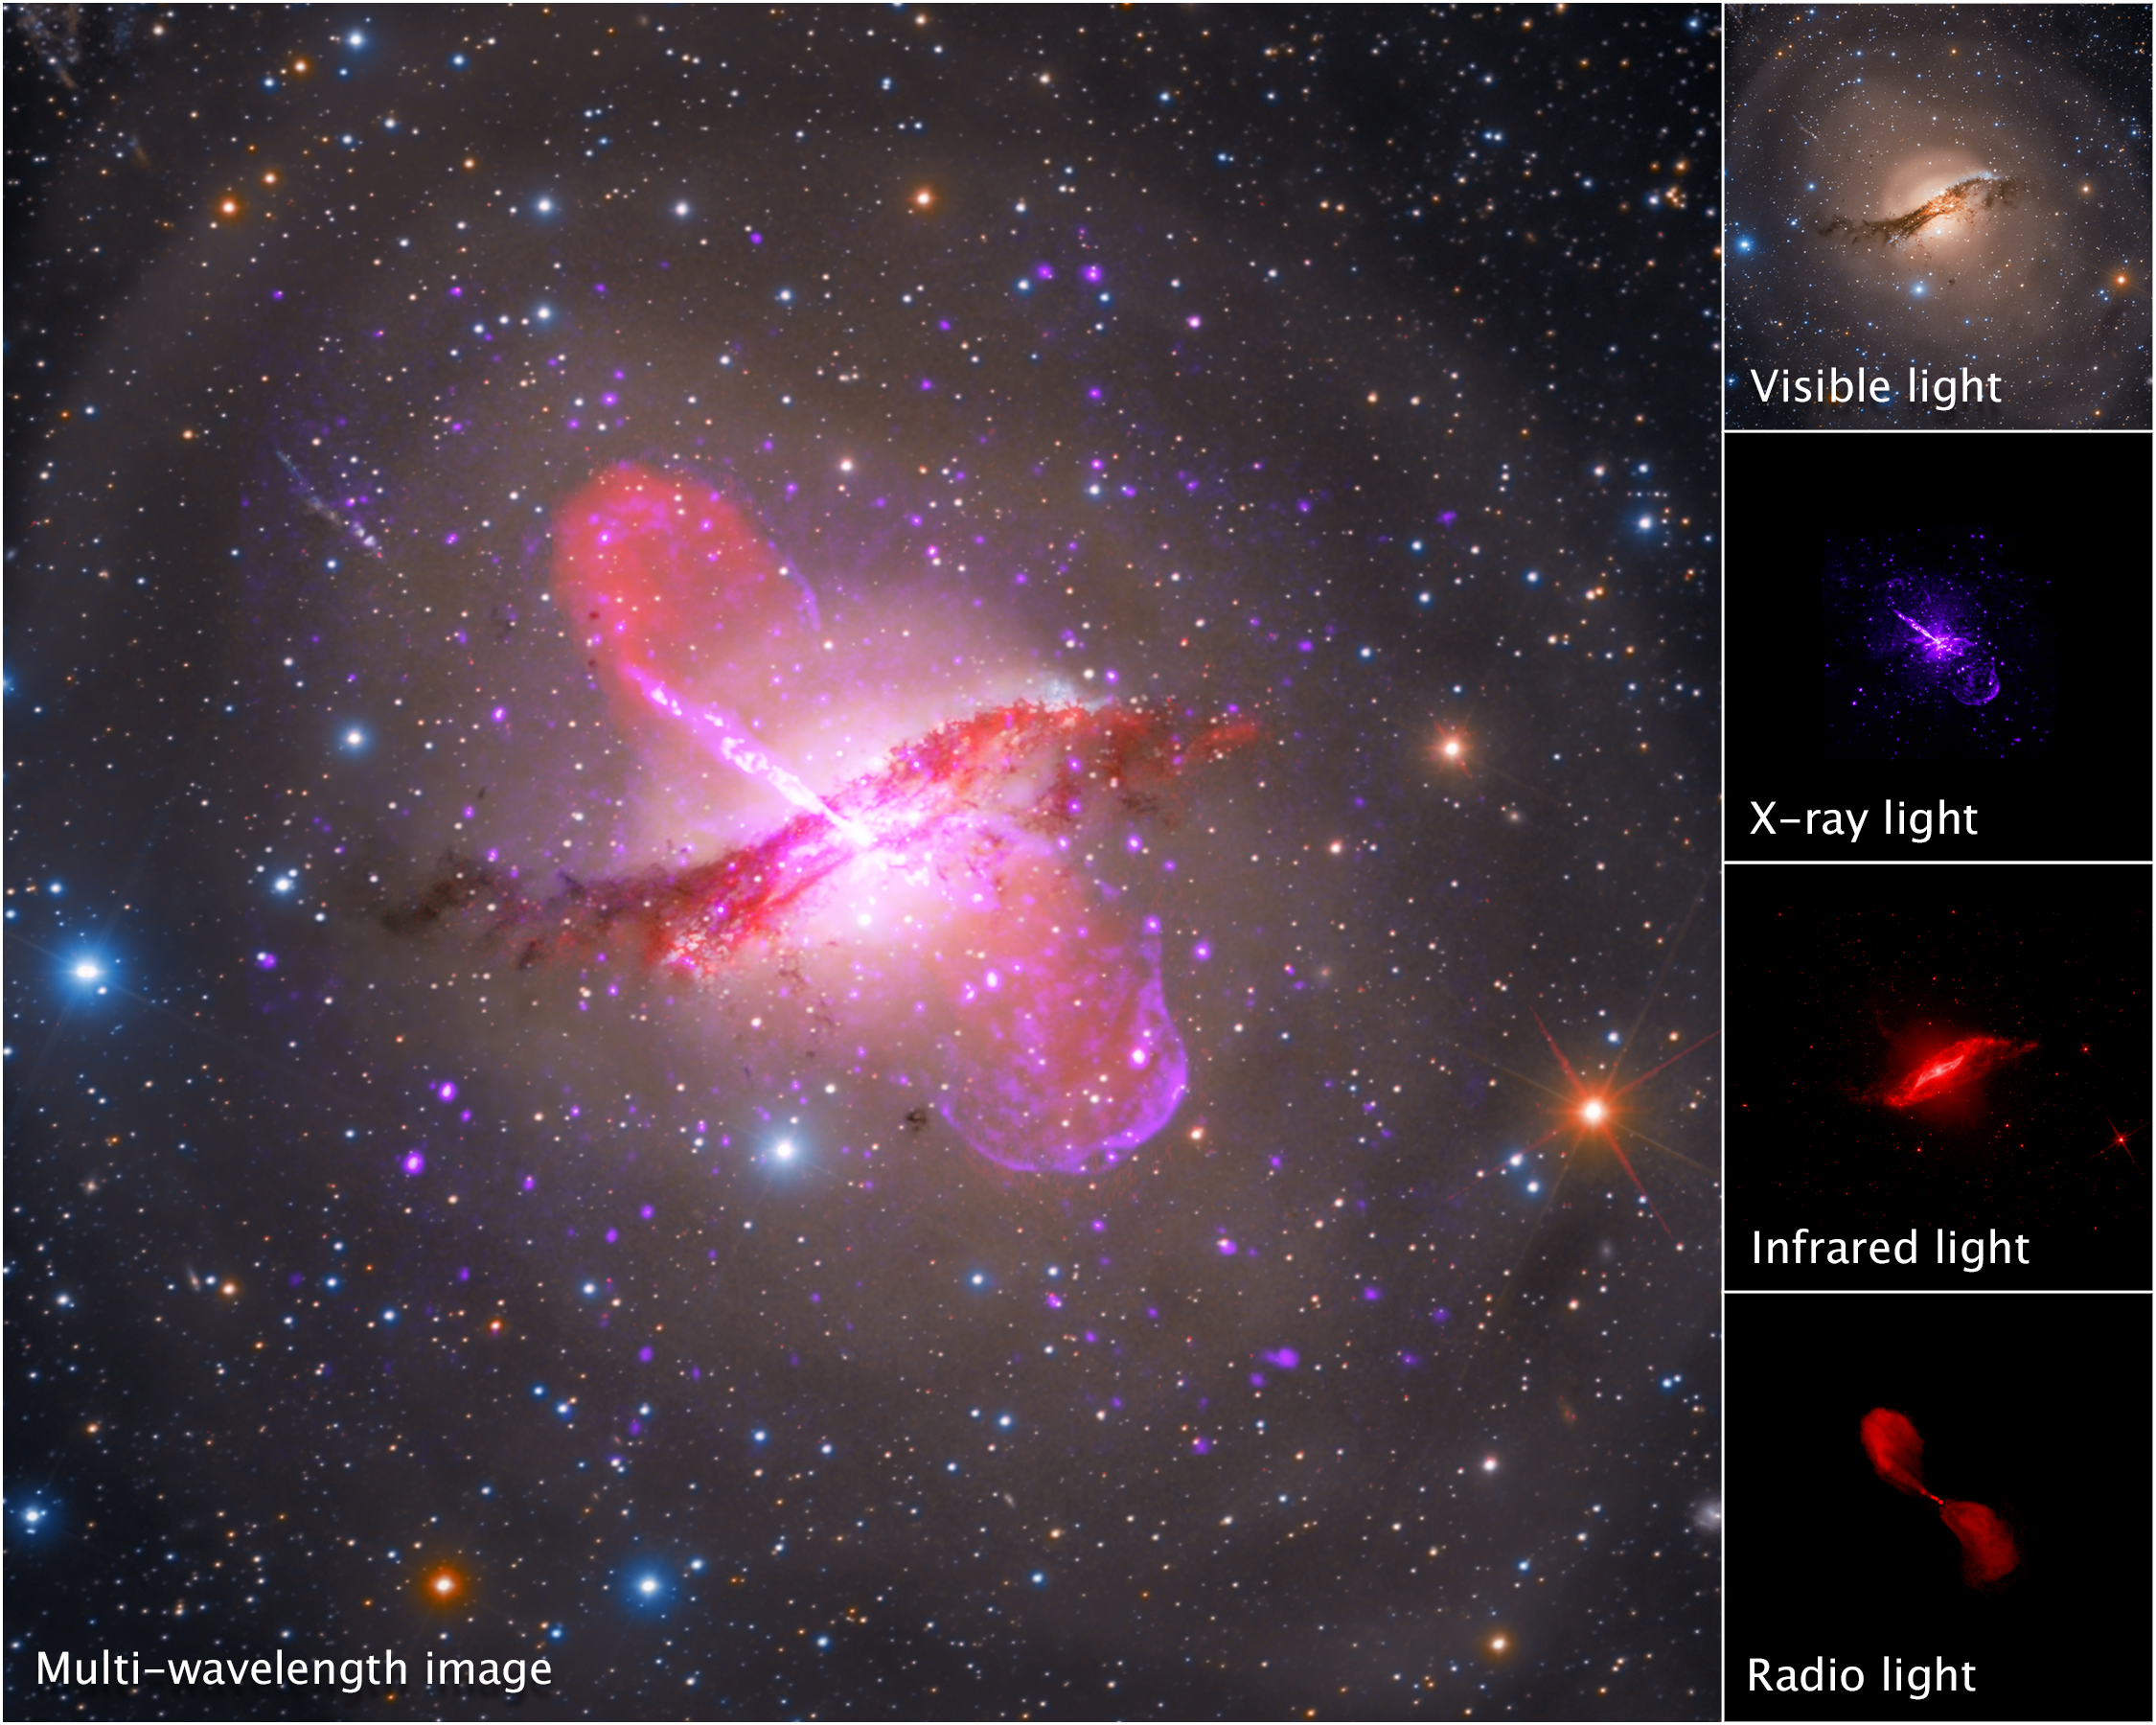
\includegraphics[width=\textwidth]{Figures/centaurusA_multiwavelength.png}
				%\caption{\tiny \textbf{Centaurus A} es una galaxia activa cercana a la Vía Láctea, ubicada a 3.5 megapársecs. Créditos: X-ray: NASA/CXC/SAO; optical: Rolf Olsen; infrared: NASA/JPL-Caltech; radio: NRAO/AUI/NSF/Univ.Hertfordshire/M.Hardcastle.}
			%\end{minipage}				
		%\end{figure}
	%\end{frame}

    %------------------------------ SLIDE ---------------------------------------
    \begin{frame}{} % cada entorno frame es una diapositiva
        \justifying % para justificar el texto, siempre al inicio de cada frame
        % Añade espacio para mover el bloque hacia arriba
        % Añade espacio para mover el bloque hacia arriba
        \vspace*{-0.5cm} % Ajusta este valor según sea necesario

        % Cuadro sin bordes redondeados, con colores personalizados
        \begin{tcolorbox}[colback=custombgcolor3, coltext=customfgcolor2,
                      colframe=custombgcolor3, % Color del borde
                      width=\textwidth,       % Ancho del cuadro
                      boxrule=1pt,            % Grosor del borde
                      top=0.1mm, bottom=0.1mm,     % Espacio superior e inferior
                      sharp corners=all,     % Bordes sin redondear
                      halign=center,         % Alineación horizontal
                      valign=center,         % Alineación vertical
                      ]
            % Texto dentro del cuadro
            \textbf{Rigidez \kern-0.9em umbral}
        \end{tcolorbox}

        \begin{columns}
            \begin{column}{0.45\textwidth} % Columna izquierda para la lista
                \begin{itemize}
                    \item Está dada por la ecuación: \[\mathbf{R} = \mathbf{\frac{pc}{Ze}},\]

                    donde $\mathbf{p}$ es el momento de la partícula, $\mathbf{c}$ es la velocidad de la luz, $\mathbf{Z}$ número de carga iónica  y $\mathbf{e}$ la carga elemental.
                    
                    \item Centro de México: $\mathbf{R_{c} \sim 8}$\textbf{.3 GV}.		
                \end{itemize}
            \end{column}
            
            \begin{column}{0.6\textwidth} % Columna derecha para la imagen
                \begin{figure}
                    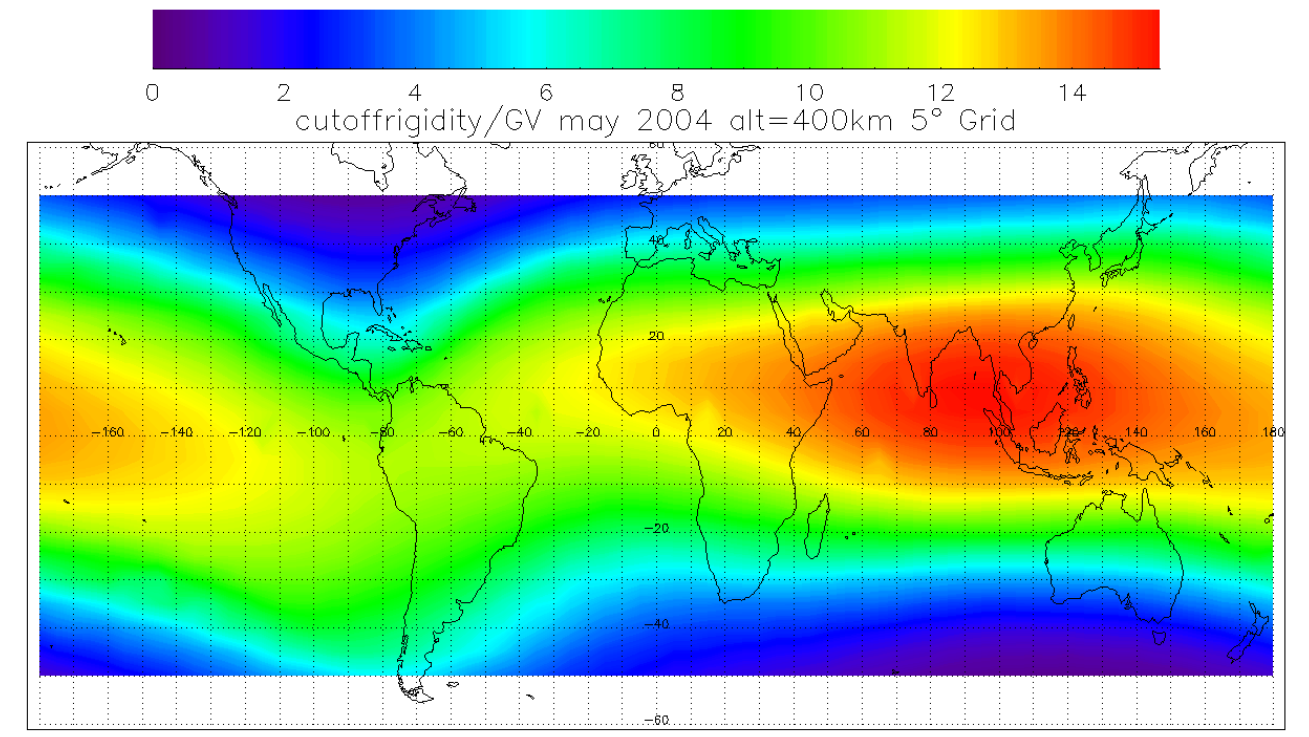
\includegraphics[width=1.0\textwidth]{Figures/rigiditymap.png}
                    \caption{\tiny Mapa de la rigidez umbral de la Tierra [\cite{labrenz2014}].}
                \end{figure}
            \end{column}
        \end{columns}
    \end{frame}   

	%------------------------------ SLIDE ---------------------------------------
    \begin{frame}{} % cada entorno frame es una diapositiva
        \justifying % para justificar el texto, siempre al inicio de cada frame
        % Añade espacio para mover el bloque hacia arriba
        % Añade espacio para mover el bloque hacia arriba
        \vspace*{-0.3cm} % Ajusta este valor según sea necesario

        % Cuadro sin bordes redondeados, con colores personalizados
        \begin{tcolorbox}[colback=custombgcolor5, coltext=customfgcolor2,
                      colframe=custombgcolor5, % Color del borde
                      width=\textwidth,       % Ancho del cuadro
                      boxrule=1pt,            % Grosor del borde
                      top=0.1mm, bottom=0.1mm,     % Espacio superior e inferior
                      sharp corners=all,     % Bordes sin redondear
                      halign=center,         % Alineación horizontal
                      valign=center,         % Alineación vertical
                      ]
            % Texto dentro del cuadro
            \textbf{Cascada \kern-0.9em de \kern-0.9em partículas}
        \end{tcolorbox}

        \vspace*{-0.5cm} % Ajusta este valor según sea necesario

        \begin{columns}
            \begin{column}{0.57\textwidth} % Columna izquierda para la lista
                \begin{itemize}
                    \item \textcolor{blue}{\textbf{Componentes:}}
                    	\begin{itemize}
                    		\item Electromagnética.
                            \item Muónica.
                            \item Hadrónica.
                    	\end{itemize}
                    		
                    \item \textcolor{blue}{\textbf{Reacciones de decaimiento:}}
                    	\begin{itemize}
                            \item $\pionnull \rightarrow 2 \gamma$
                            \item $\pionplus \rightarrow \antimuon + \neutrino$
                            \item $\pionminus \rightarrow \muon + \antineutrino$
                    	\end{itemize}
                    \item \textcolor{blue}{\textbf{\small Vida media $\pionnull$:}} \small $\sim 10^{-16}$ s.
                    \item \textcolor{blue}{\textbf{\small Vida media de los piones ($\pionplus$ y $\pionminus$):}} \small $\sim 26$ ns.
                \end{itemize}
            \end{column}

            \begin{column}{0.5\textwidth} % Columna derecha para la imagen
                \begin{figure}
                    \centering
                    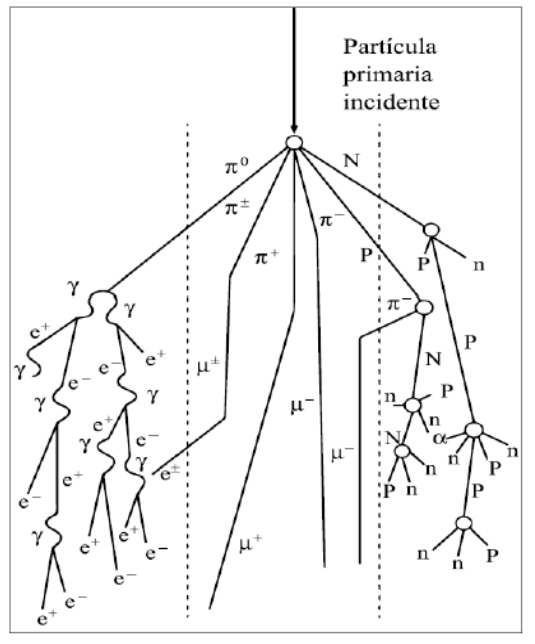
\includegraphics[width=0.8\textwidth]{Figures/showercomponent.png}
                    \caption{\tiny Esquema de las componentes de un chubasco de partículas [\cite{valdesgalicia1992}].}
                \end{figure}
            \end{column}
        \end{columns}
    \end{frame}     

    %------------------------------ SLIDE ---------------------------------------
    %\begin{frame}{} % cada entorno frame es una diapositiva
        %\justifying % para justificar el texto, siempre al inicio de cada frame
        % Añade espacio para mover el bloque hacia arriba
        % Añade espacio para mover el bloque hacia arriba
        %\vspace*{-0.1cm} % Ajusta este valor según sea necesario
        
        % Cuadro sin bordes redondeados, con colores personalizados
        %\begin{tcolorbox}[colback=custombgcolor6, coltext=customfgcolor2,
                      %colframe=custombgcolor6, % Color del borde
                      %width=\textwidth,       % Ancho del cuadro
                      %boxrule=1pt,            % Grosor del borde
                      %top=1mm, bottom=1mm,     % Espacio superior e inferior
                      %sharp corners=all,     % Bordes sin redondear
                      %halign=center,         % Alineación horizontal
                      %valign=center,         % Alineación vertical
                      %]
            % Texto dentro del cuadro
            %\textbf{Componente \kern-0.9em hadrónica}
        %\end{tcolorbox}
        
        %\begin{figure}
        	%\centering
        	%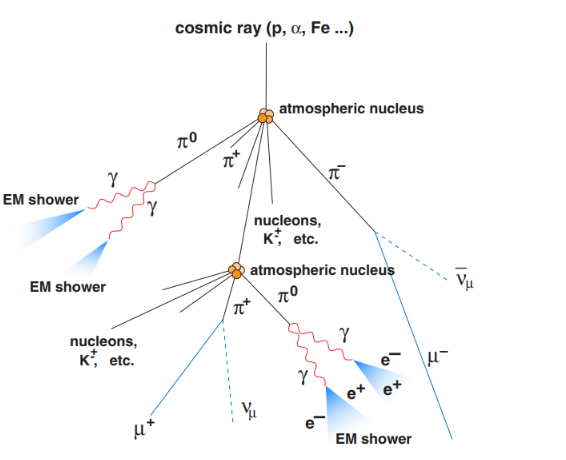
\includegraphics[width=0.5\textwidth]{Figures/hadronicshower.png}
        %\end{figure}
    %\end{frame}

    %------------------------------ SLIDE ---------------------------------------
    %\begin{frame}{} % cada entorno frame es una diapositiva
        %\justifying % para justificar el texto, siempre al inicio de cada frame
        % Añade espacio para mover el bloque hacia arriba
        % Añade espacio para mover el bloque hacia arriba
        %\vspace*{-0.2cm} % Ajusta este valor según sea necesario

        % Cuadro sin bordes redondeados, con colores personalizados
        %\begin{tcolorbox}[colback=custombgcolor3, coltext=customfgcolor2,
                      %colframe=custombgcolor3, % Color del borde
                      %width=\textwidth,       % Ancho del cuadro
                      %boxrule=1pt,            % Grosor del borde
                      %top=1mm, bottom=1mm,     % Espacio superior e inferior
                      %sharp corners=all,     % Bordes sin redondear
                      %halign=center,         % Alineación horizontal
                      %valign=center,         % Alineación vertical
                      %]
            % Texto dentro del cuadro
            %\textbf{Componente \kern-0.9em muónica}
        %\end{tcolorbox}
        
        %Reacciones más importantes:
		
		%\[
		%\begin{split}
		%\pionplus \rightarrow \antimuon + \neutrino, \\
		%\pionminus \rightarrow \muon + \antineutrino, \\
		%\pionnull \rightarrow 2 \gamma.
		%\end{split}
		%\]
		
		%\[
		%\begin{split}
		%\Kaonplus \rightarrow \antimuon + \neutrino, \\
		%\Kaonminus \rightarrow \muon + \antineutrino.
		%\end{split}
		%\]

        %\begin{columns}
            %\begin{column}{1.0\textwidth} % Columna izquierda para la lista
                %\begin{itemize}
                    %\item Vida media de los piones ($\pionplus$ y $\pionminus$): $2.6 \times 10^{-8}$s. 
                    %\item Vida media de los kaones ($\Kaonplus$ y $\Kaonminus$): $\sim 10^{-8}$ y $10^{-11}$s.
                %\end{itemize}
            %\end{column}
        %\end{columns} 
    %\end{frame}       
    
    %------------------------------ SLIDE ---------------------------------------
    %\begin{frame}{} % cada entorno frame es una diapositiva
        %\justifying % para justificar el texto, siempre al inicio de cada frame
        % Añade espacio para mover el bloque hacia arriba
        % Añade espacio para mover el bloque hacia arriba
        %\vspace*{-0.1cm} % Ajusta este valor según sea necesario
        
        % Cuadro sin bordes redondeados, con colores personalizados
        %\begin{tcolorbox}[colback=custombgcolor8, coltext=customfgcolor2,
                      %colframe=custombgcolor8, % Color del borde
                      %width=\textwidth,       % Ancho del cuadro
                      %boxrule=1pt,            % Grosor del borde
                      %top=1mm, bottom=1mm,     % Espacio superior e inferior
                      %sharp corners=all,     % Bordes sin redondear
                      %halign=center,         % Alineación horizontal
                      %valign=center,         % Alineación vertical
                      %]
            % Texto dentro del cuadro
            %\textbf{Componente \kern-0.9em electromagnética}
        %\end{tcolorbox}
        
        %\begin{figure}
        	%\centering
        	%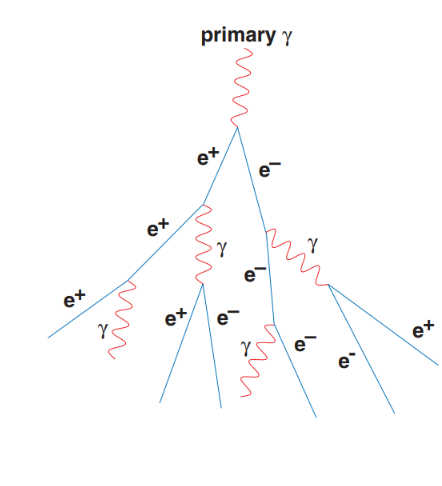
\includegraphics[width=0.4\textwidth]{Figures/electromagshower.png}
        %\end{figure}
    %\end{frame} 
    
	%------------------------------ SLIDE --------------------------------------- ORIGINAL METODOS DE DETECCION
    %\begin{frame}{} % cada entorno frame es una diapositiva
        %\justifying % para justificar el texto, siempre al inicio de cada frame
        % Añade espacio para mover el bloque hacia arriba
        % Añade espacio para mover el bloque hacia arriba
        %\vspace*{-0.3cm} % Ajusta este valor según sea necesario

        % Cuadro sin bordes redondeados, con colores personalizados
        %\begin{tcolorbox}[colback=custombgcolor3, coltext=customfgcolor2,
                      %colframe=custombgcolor3, % Color del borde
                      %width=\textwidth,       % Ancho del cuadro
                      %boxrule=1pt,            % Grosor del borde
                      %top=1mm, bottom=1mm,     % Espacio superior e inferior
                      %sharp corners=all,     % Bordes sin redondear
                      %halign=center,         % Alineación horizontal
                      %valign=center,         % Alineación vertical
                      %]
            % Texto dentro del cuadro
            %\textbf{Métodos \kern-0.9em de \kern-0.9em detección}
            %\textcolor{black}{\textbf{Métodos \kern-0.9em de \kern-0.9em detección}}        
        %\end{tcolorbox}

        %\begin{columns}
            %\begin{column}{0.45\textwidth} % Columna izquierda para la lista
                %\begin{itemize}
                    %\item \textcolor{blue}{\textbf{Detección directa:}}
                    	%\begin{itemize}
                    		%\item naves espaciales.
                            %\item satélites.
                    	%\end{itemize}
                    		
                    %\item \textcolor{blue}{\textbf{Detección indirecta:}}
                    	%\begin{itemize}
                    		%\item detectores Cherenkov.
                    		%\item neutrones.
                    		%\item muones.
                    	%\end{itemize}
                %\end{itemize}
            %\end{column}

            %\begin{column}{0.4\textwidth} % Columna derecha para la imagen
                %\begin{figure}
                    %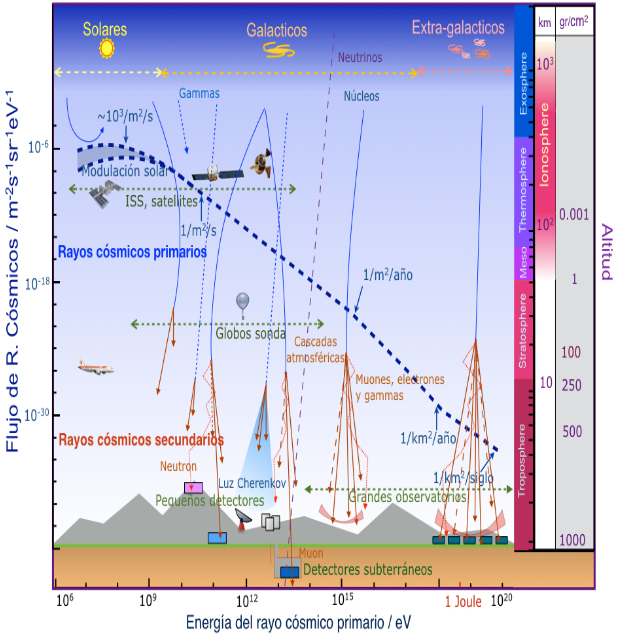
\includegraphics[width=0.8\textwidth]{Figures/spectrum2.png}
                    %\caption{\tiny Espectro de los RC, se muestra los instrumentos usados para la detección a diferentes altitudes. Imagen tomada del \href{https://revista.iaa.csic.es/content/portada/404/69}{Instituto de Astrofísica de Andalucía (IAA-CSIC)} (2023).} 
                %\end{figure}               
            %\end{column}
        %\end{columns}
    %\end{frame} 
    
	%------------------------------ SLIDE ---------------------------------------
    %\begin{frame}{} % cada entorno frame es una diapositiva
        %\justifying % para justificar el texto, siempre al inicio de cada frame
        % Añade espacio para mover el bloque hacia arriba
        % Añade espacio para mover el bloque hacia arriba
        %\vspace*{-1.5cm} % Ajusta este valor según sea necesario

        % Cuadro sin bordes redondeados, con colores personalizados
        %\begin{tcolorbox}[colback=custombgcolor9, coltext=customfgcolor2,
                      %colframe=custombgcolor9, % Color del borde
                      %width=\textwidth,       % Ancho del cuadro
                      %boxrule=1pt,            % Grosor del borde
                      %top=1mm, bottom=1mm,     % Espacio superior e inferior
                      %sharp corners=all,     % Bordes sin redondear
                      %halign=center,         % Alineación horizontal
                      %valign=center,         % Alineación vertical
                      %]
            % Texto dentro del cuadro
            %\textbf{Observatorios \kern-0.5em de \kern-0.5em Rayos \kern-0.5em Cósmicos \kern-0.5em en \kern-0.5em Sierra \kern-0.5em Negra}
            %\textcolor{black}{\textbf{Observatorios \kern-0.5em de \kern-0.5em Rayos \kern-0.5em Cósmicos \kern-0.5em en \kern-0.5em Sierra \kern-0.5em Negra}}
        %\end{tcolorbox}

        %\begin{columns}
            %\begin{column}{0.6\textwidth} % Columna izquierda para la lista
                %\begin{itemize}
                    %\item \textcolor{blue}{\textbf{Telescopio de Neutrones Solares (TNS):}}
                    	%\begin{itemize}
                    		%\item Instalado por el \emph{Instituto de Geofísica} (UNAM).
                            %\item Mide la energía y dirección de las partículas.
                            %\item Forma parte de la red global de TNS.
                    	%\end{itemize}
                %\end{itemize}
            %\end{column}

            %\begin{column}{0.4\textwidth} % Columna derecha para la imagen
                %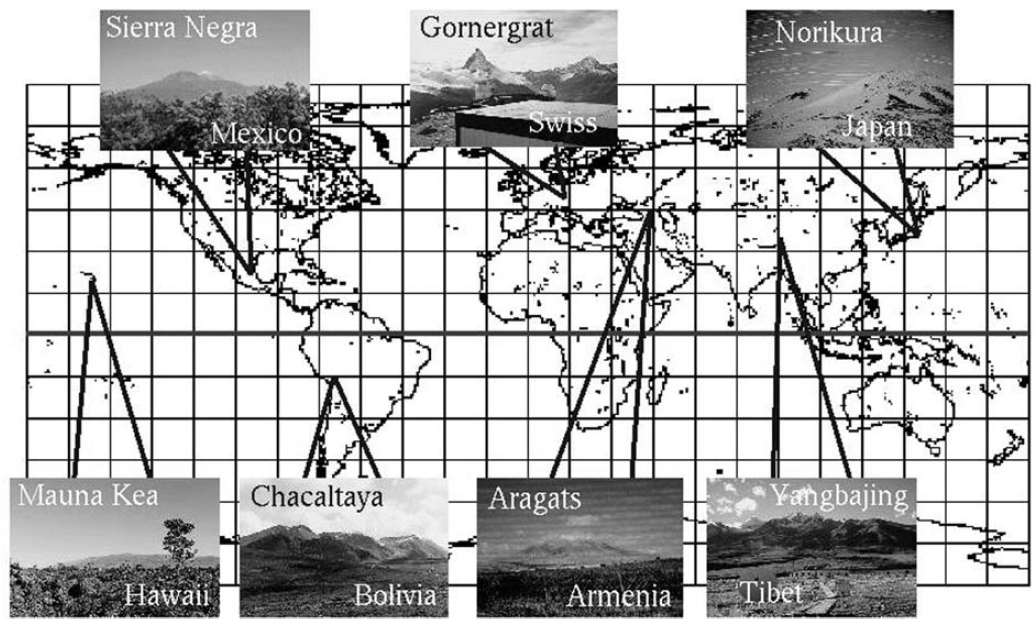
\includegraphics[width=1.0\textwidth]{Figures/TNS_NETWORK.png}
            %\end{column}
        %\end{columns}
    %\end{frame} 

	%------------------------------ SLIDE ---------------------------------------
    %\begin{frame}{} % cada entorno frame es una diapositiva
        %\justifying % para justificar el texto, siempre al inicio de cada frame
        % Añade espacio para mover el bloque hacia arriba
        % Añade espacio para mover el bloque hacia arriba
        %\vspace*{-1.5cm} % Ajusta este valor según sea necesario

        %\begin{columns}
            %\begin{column}{0.6\textwidth} % Columna izquierda para la lista
                %\begin{itemize}
                    %\item \textcolor{blue}{\textbf{Telescopio de centelleo de Rayos Cósmicos:}}
                    	%\begin{itemize}
                    		%\item Detección de neutrones solares.
                                %\item Rayos gamma.
                                %\item Muones.
                    	%\end{itemize}
                %\end{itemize}
            %\end{column}

            %\begin{column}{0.3\textwidth} % Columna derecha para la imagen
                %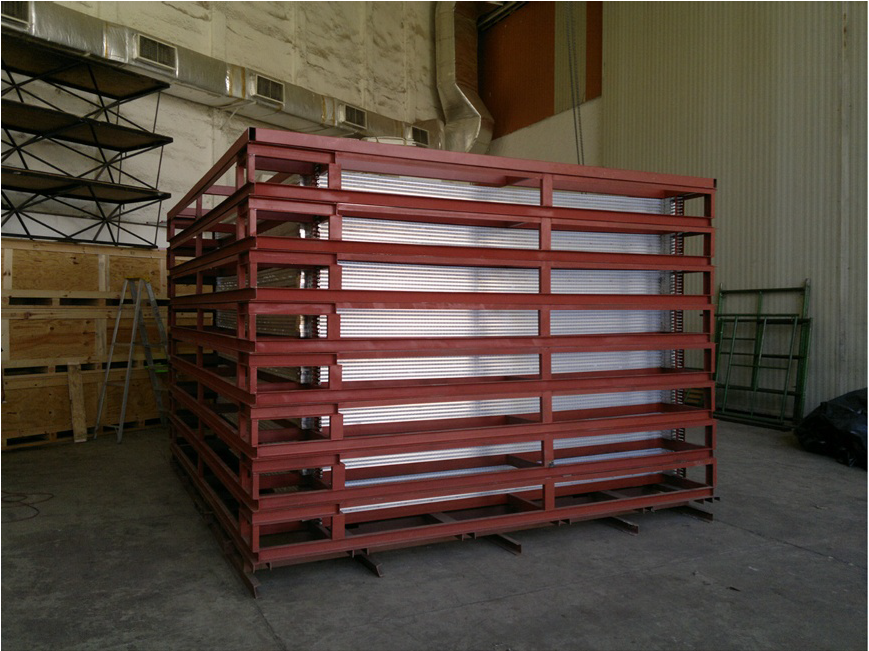
\includegraphics[width=1.2\textwidth]{Figures/scicrt-real.png}
            %\end{column}
        %\end{columns}
    %\end{frame}

	%------------------------------ SLIDE ---------------------------------------
    %\begin{frame}{} % cada entorno frame es una diapositiva
        %\justifying % para justificar el texto, siempre al inicio de cada frame
        % Añade espacio para mover el bloque hacia arriba
        % Añade espacio para mover el bloque hacia arriba
        %\vspace*{-1.5cm} % Ajusta este valor según sea necesario

        %\begin{columns}
            %\begin{column}{0.4\textwidth} % Columna izquierda para la lista
                %\begin{itemize}
                    %\item \textcolor{blue}{\textbf{HAW (High Altitude Water Cherenkov):}}
                    	%\begin{itemize}
                    		%\item 300 tanques cilíndricos.
                            %\item Detección de rayos gamma.
                            %\item Detección de rayos cósmicos en un rango de energía de TeV.
                    	%\end{itemize}
                %\end{itemize}
            %\end{column}

            %\begin{column}{0.4\textwidth} % Columna derecha para la imagen
                %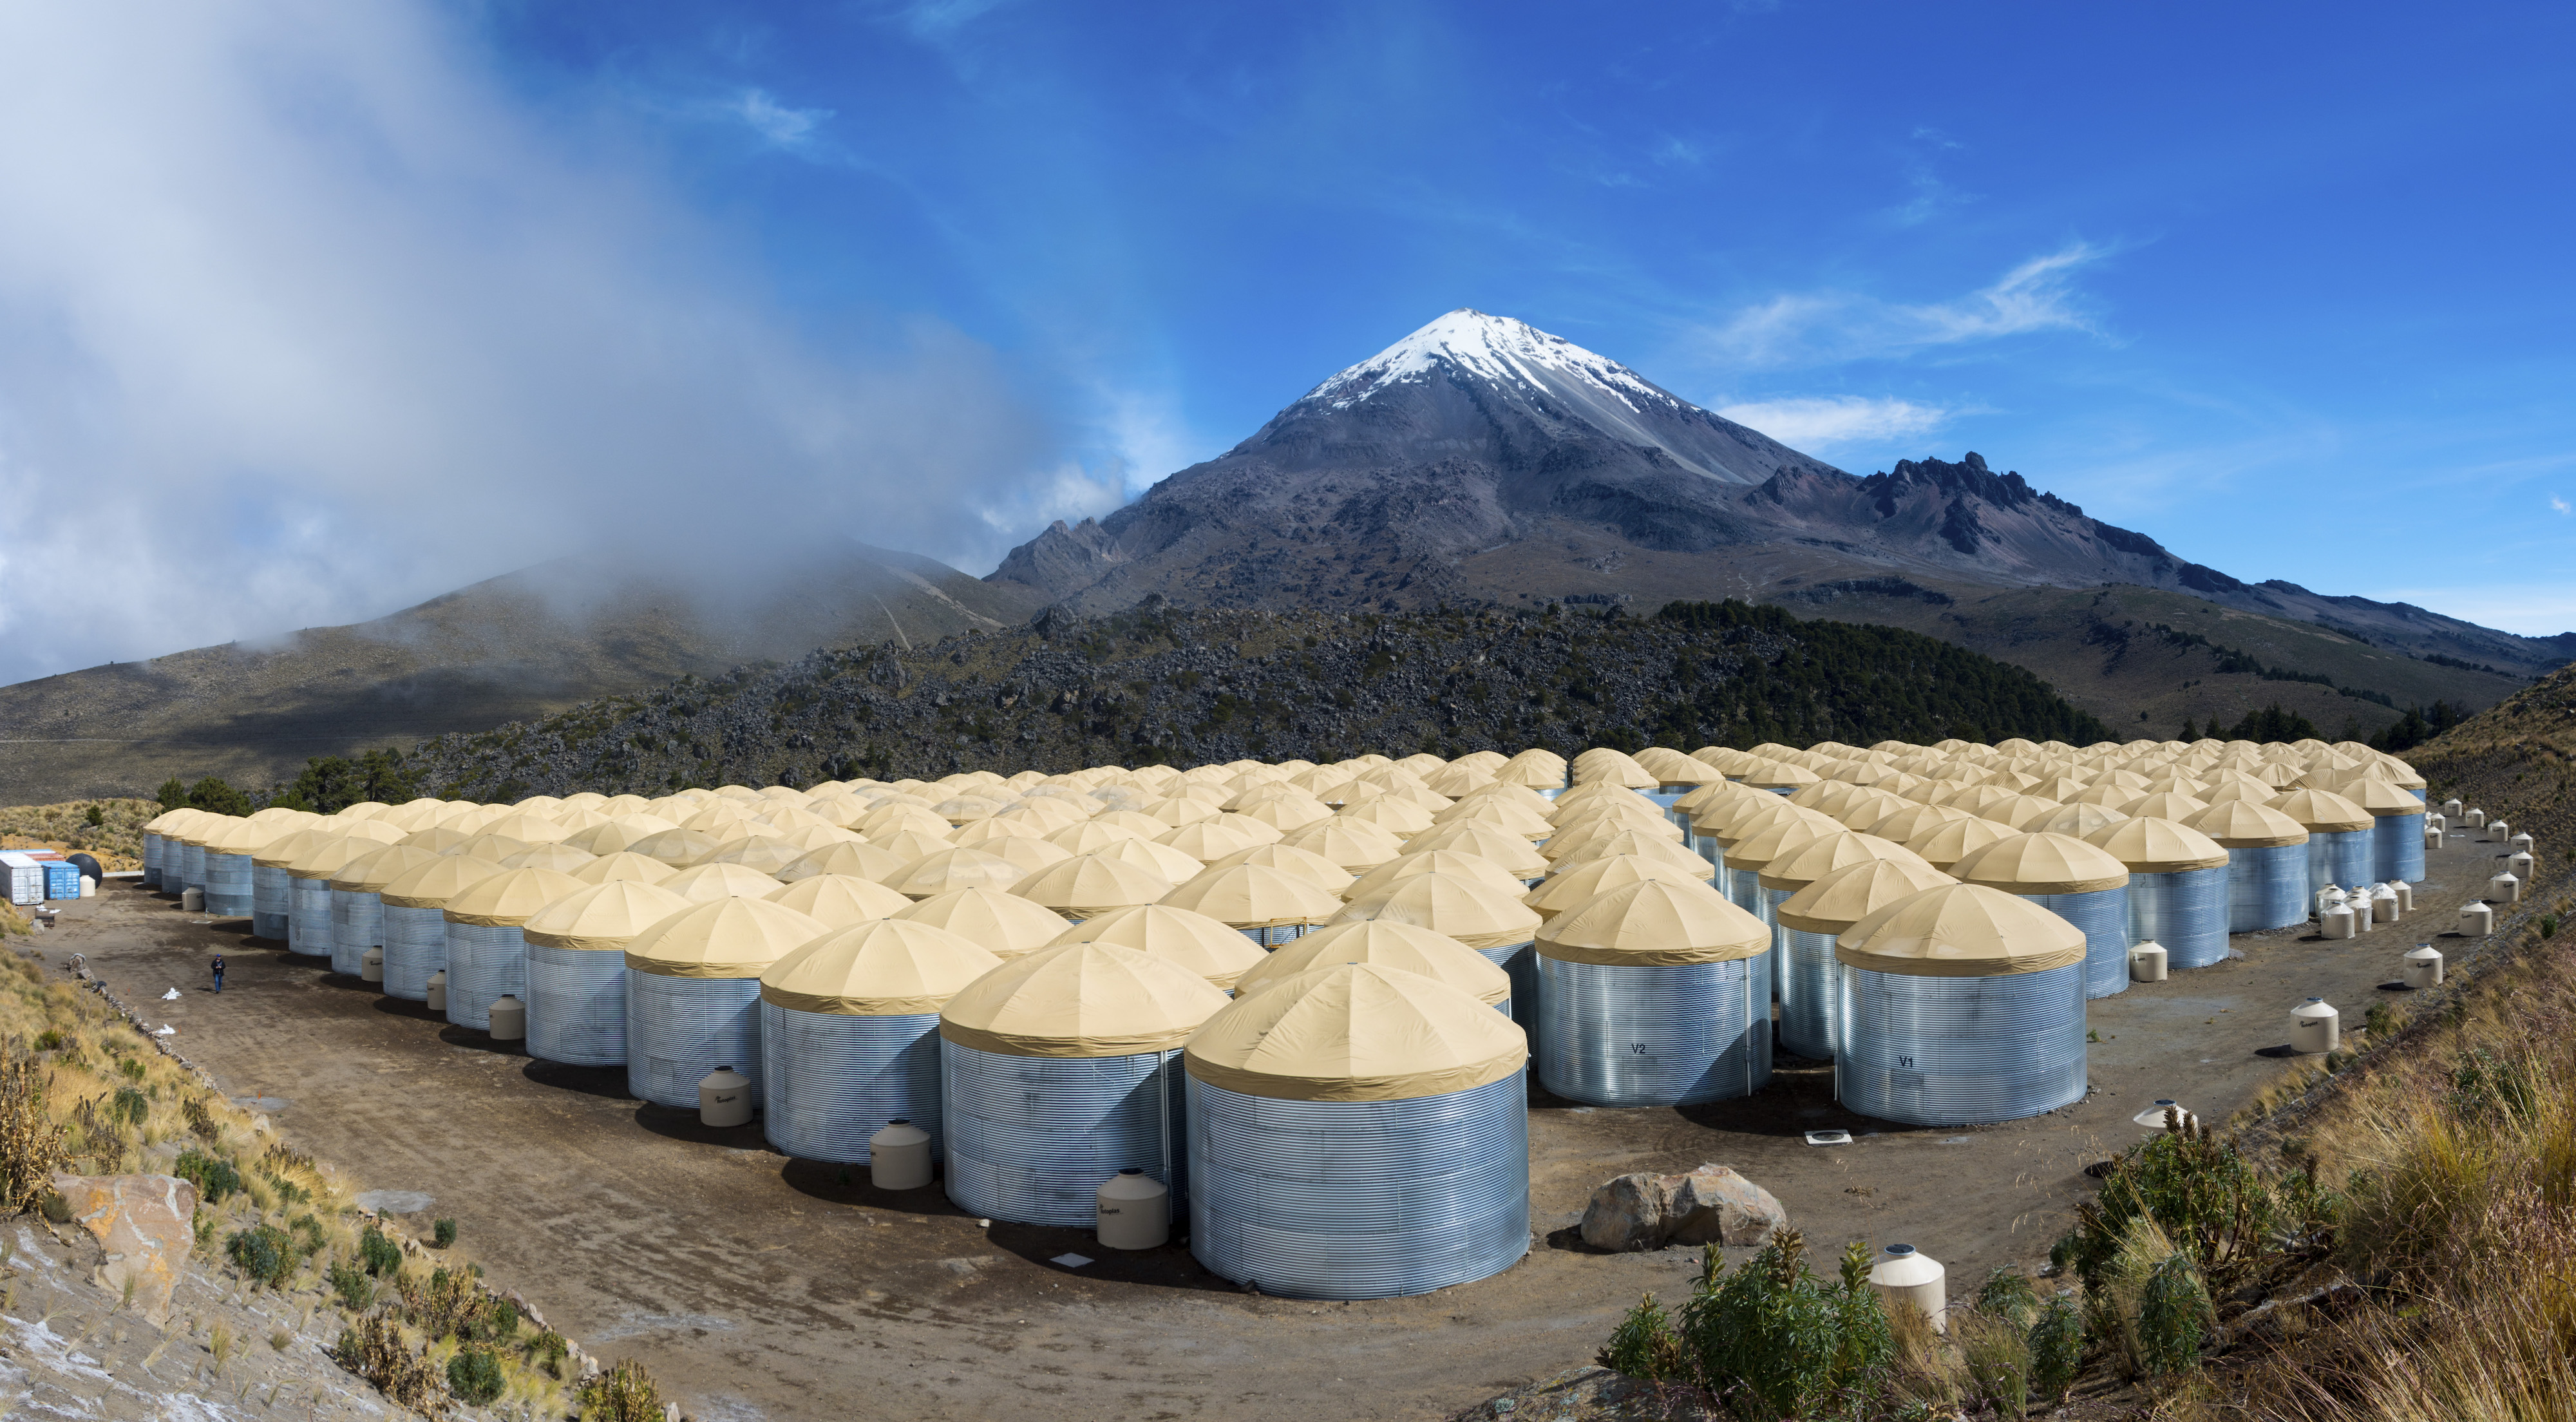
\includegraphics[width=1.1\textwidth]{Figures/hawc-real.jpg}
            %\end{column}
        %\end{columns}
    %\end{frame}

	%------------------------------ SLIDE ---------------------------------------
    %\begin{frame}{} % cada entorno frame es una diapositiva
        %\justifying % para justificar el texto, siempre al inicio de cada frame
        % Añade espacio para mover el bloque hacia arriba
        % Añade espacio para mover el bloque hacia arriba
        %\vspace*{-1.5cm} % Ajusta este valor según sea necesario

        %\begin{columns}
            %\begin{column}{0.4\textwidth} % Columna izquierda para la lista
                %\begin{itemize}
                    %\item \textcolor{blue}{\textbf{Mini Monitor de Neutrones (MNM):}}
                    	%\begin{itemize}
                    		%\item Tasa de conteo en función de la rigidez de corte $\mathbf{R_{c}}$.
                            %\item Adquirido por el Instituto de Geofísica UNAM.
                            %\item Funciona con el gas $\ce{^{10}BF_{3}}$.
                            %\item Facilita su movilidad debido a su tamaño reducido. 
                    	%\end{itemize}
                %\end{itemize}
            %\end{column}

            %\begin{column}{0.4\textwidth} % Columna derecha para la imagen
                %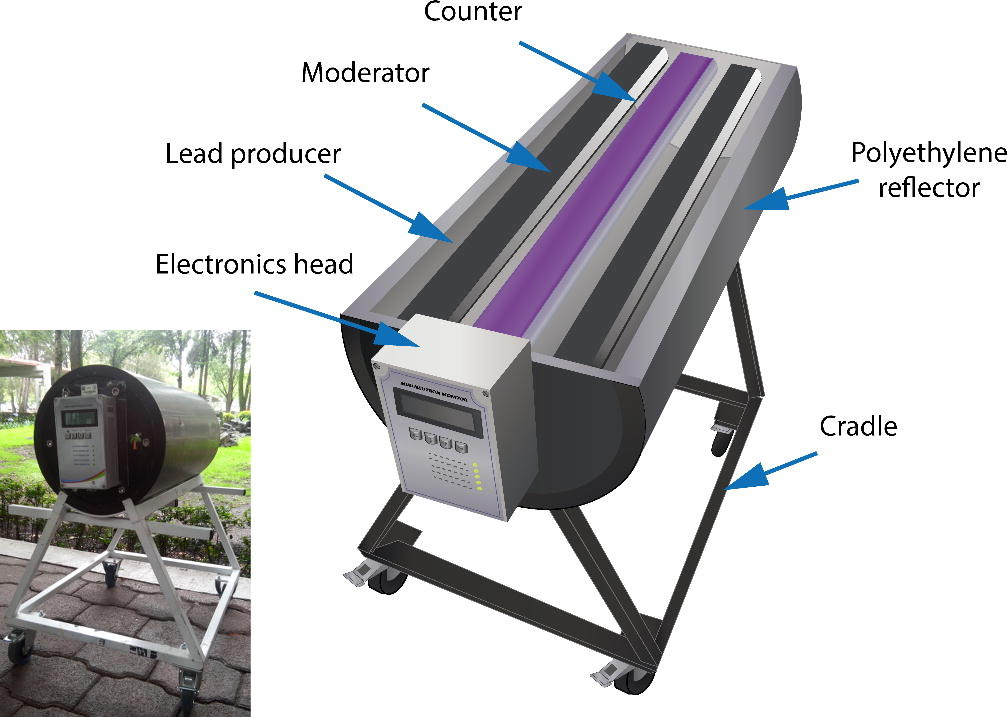
\includegraphics[width=1.1\textwidth]{Figures/detector1.jpg}
            %\end{column}
        %\end{columns}
    %\end{frame}

	%------------------------------ SLIDE ---------------------------------------
    \begin{frame}{} % cada entorno frame es una diapositiva
        \justifying % para justificar el texto, siempre al inicio de cada frame
        % Añade espacio para mover el bloque hacia arriba
        % Añade espacio para mover el bloque hacia arriba
        \vspace*{-0.3cm} % Ajusta este valor según sea necesario

        % Cuadro sin bordes redondeados, con colores personalizados
        \begin{tcolorbox}[colback=custombgcolor9, coltext=customfgcolor2,
                      colframe=custombgcolor9, % Color del borde
                      width=\textwidth,       % Ancho del cuadro
                      boxrule=1pt,            % Grosor del borde
                      top=0.1mm, bottom=0.1mm,     % Espacio superior e inferior
                      sharp corners=all,     % Bordes sin redondear
                      halign=center,         % Alineación horizontal
                      valign=center,         % Alineación vertical
                      ]
            % Texto dentro del cuadro
            \textbf{Observatorios \kern-0.5em de \kern-0.5em Rayos \kern-0.5em Cósmicos \kern-0.5em en \kern-0.5em Sierra \kern-0.5em Negra}
        \end{tcolorbox}        

        \begin{columns}
            \begin{column}{0.5\textwidth} % Columna izquierda para la lista
                \begin{itemize}
                    \item \textcolor{blue}{\textbf{HAWC (High Altitude Water Cherenkov)}}
                     \begin{figure}
                         \centering
                         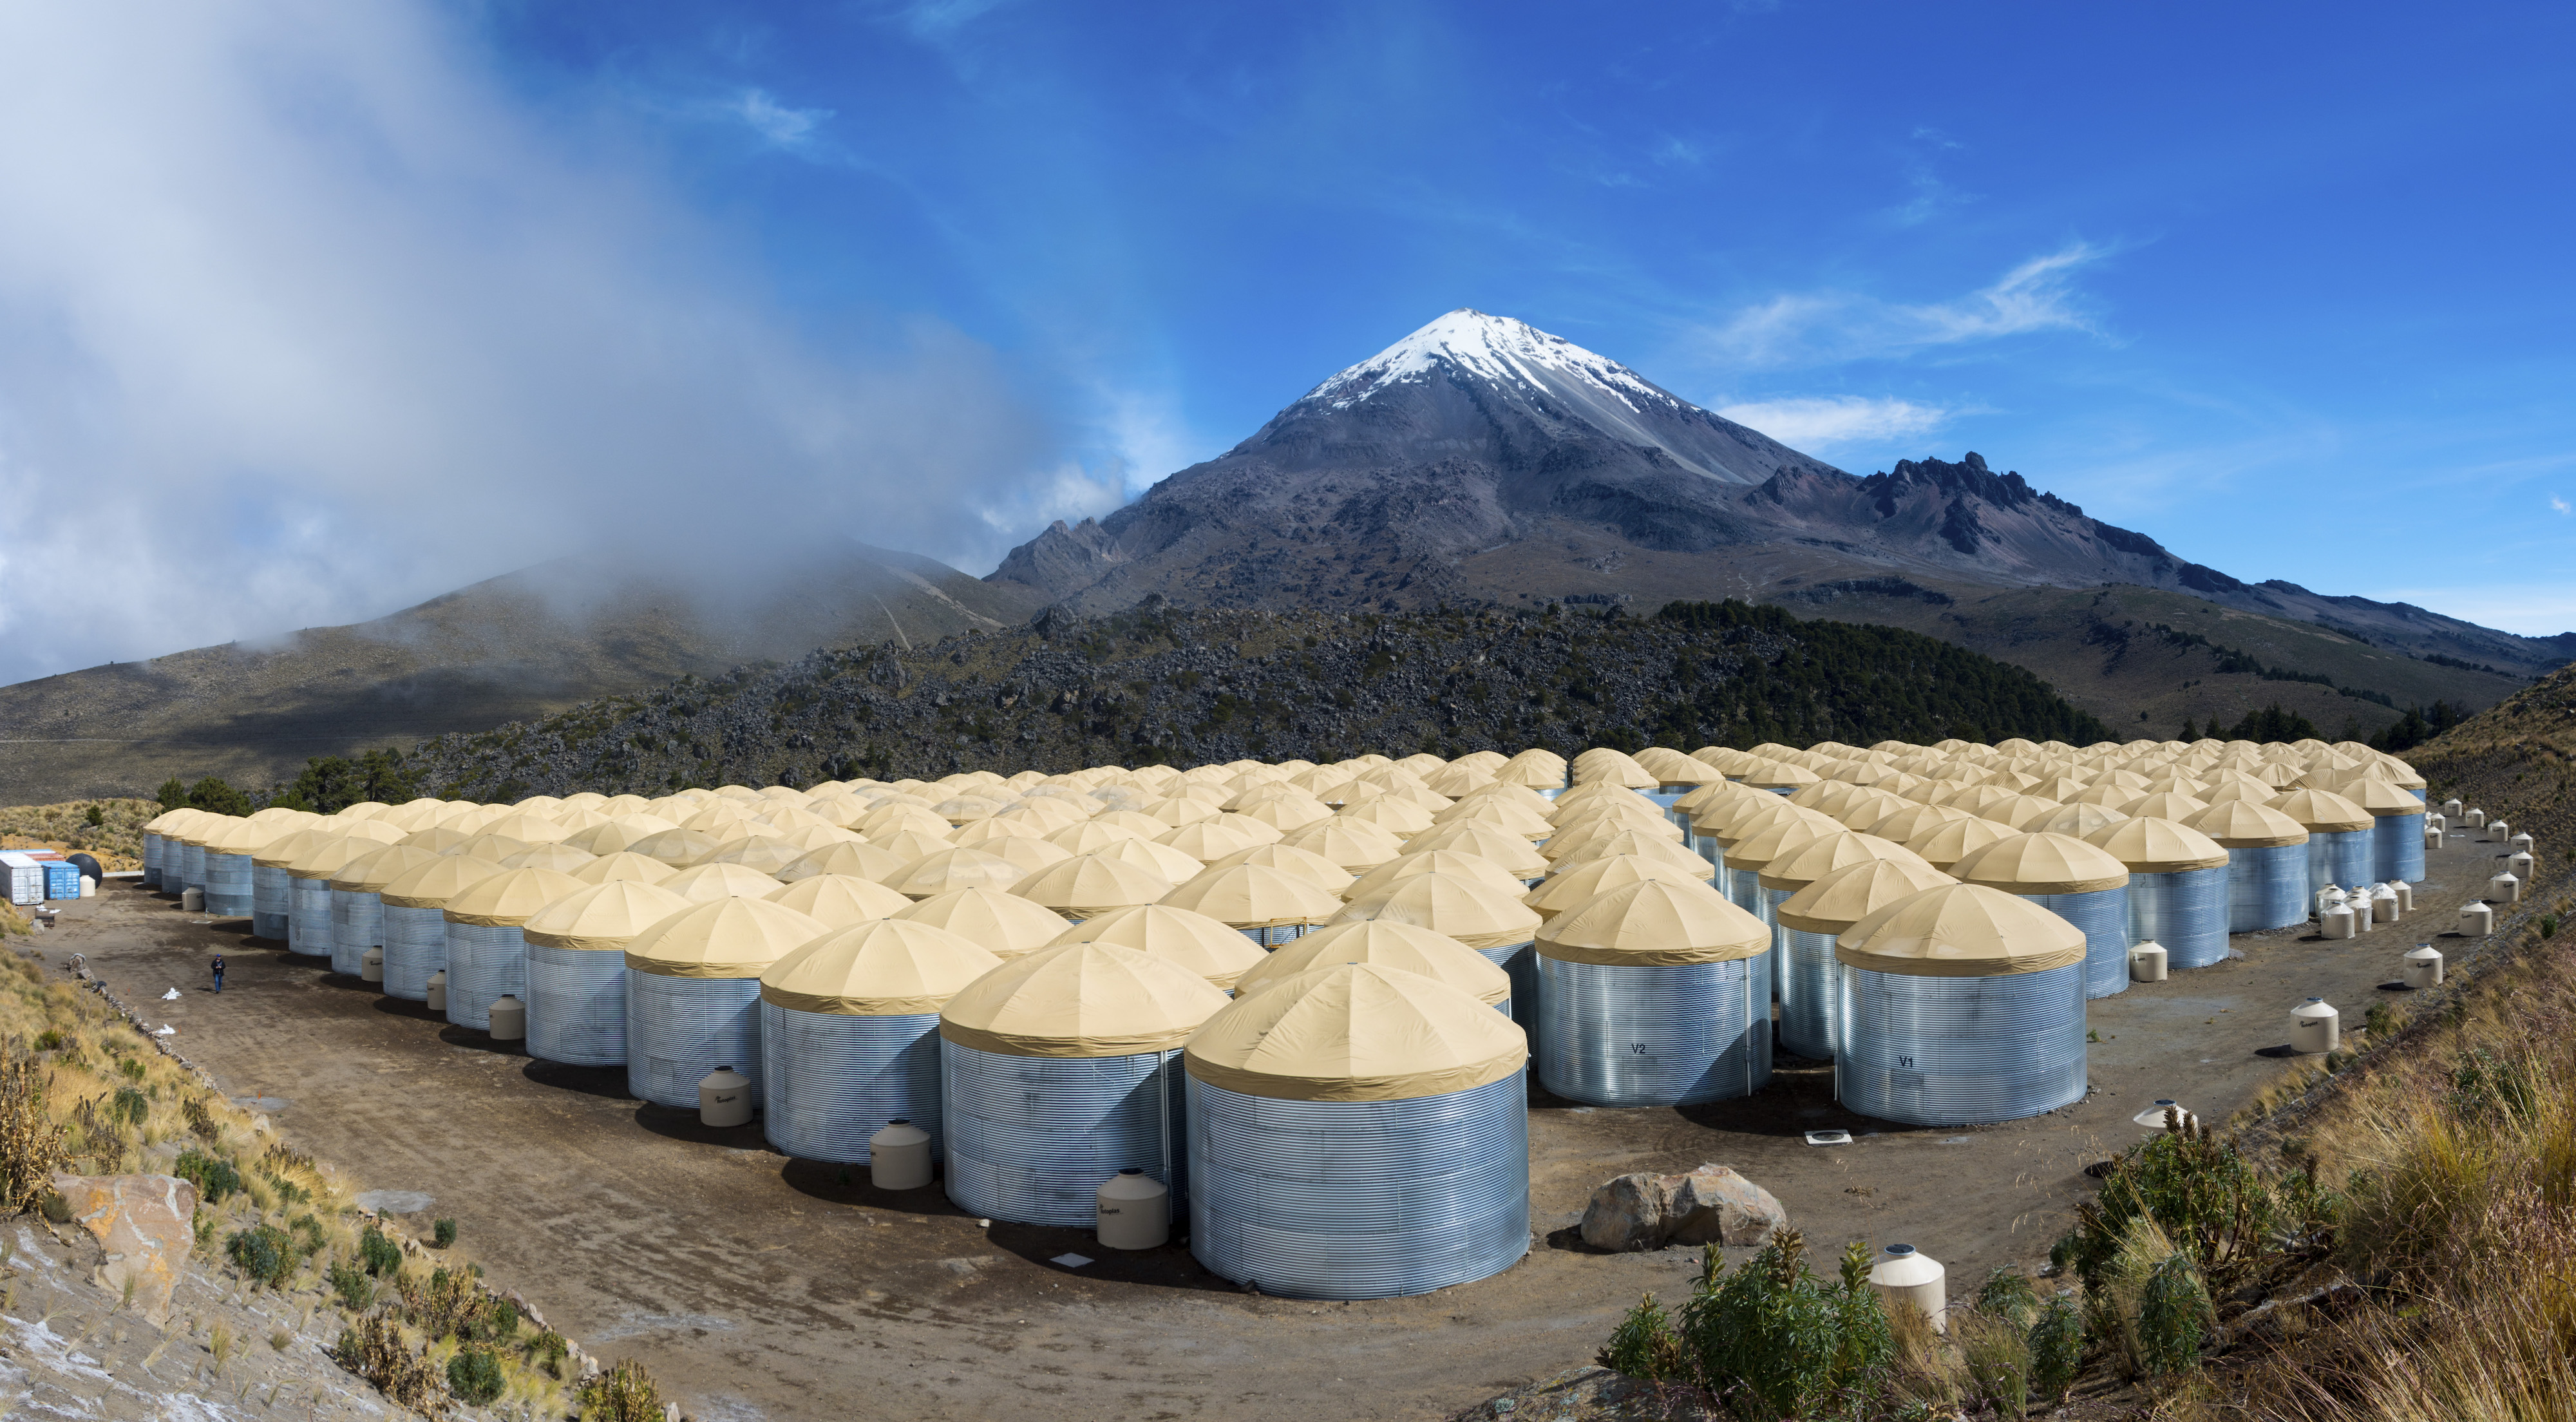
\includegraphics[width=0.65\linewidth]{Figures/hawc-real.jpg}
                     \end{figure}

                     \item \textcolor{blue}{\textbf{Mini Monitor de Neutrones portátil (MNM)}}
                     \begin{figure}
                         \centering
                         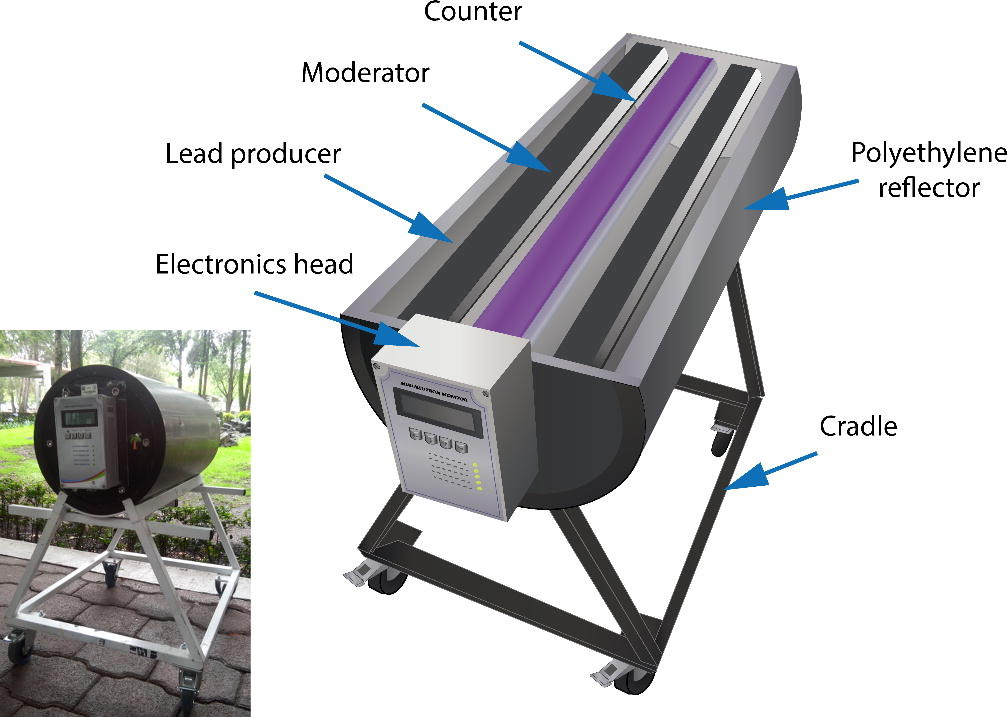
\includegraphics[width=0.6\linewidth]{Figures/detector1.jpg}
                     \end{figure}                     
                \end{itemize}
            \end{column}

            \begin{column}{0.5\textwidth} % Columna izquierda para la lista
                \begin{itemize}
                    \item \textcolor{blue}{\textbf{Telescopio de Centelleo de Rayos Cósmicos (SciCRT)}}
                     \begin{figure}
                         \centering
                         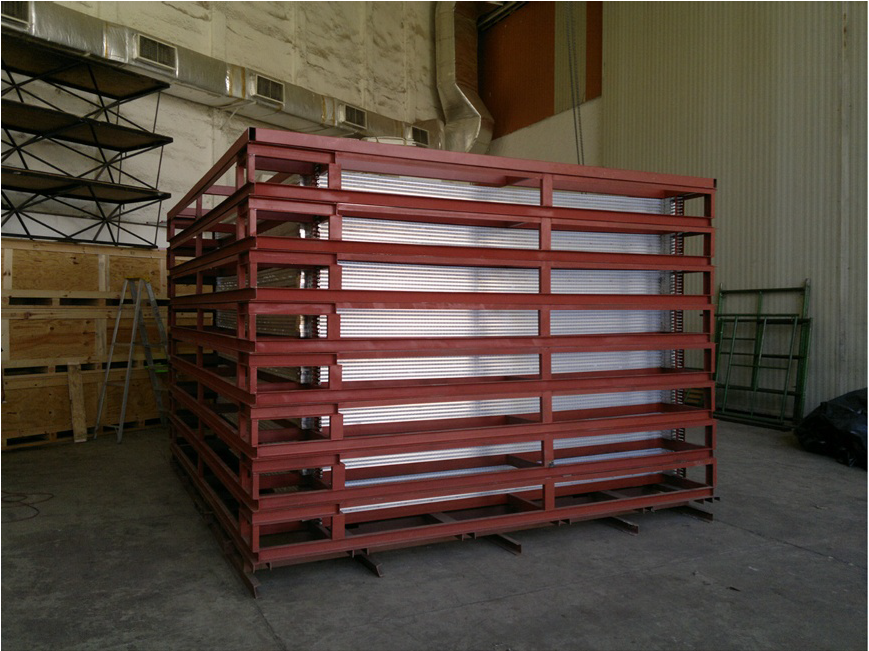
\includegraphics[width=0.5\linewidth]{Figures/scicrt-real.png}
                     \end{figure}

                     \item \textcolor{blue}{\textbf{Telescopio de Neutrones Solares (TNS)}}
                     \begin{figure}
                         \centering
                         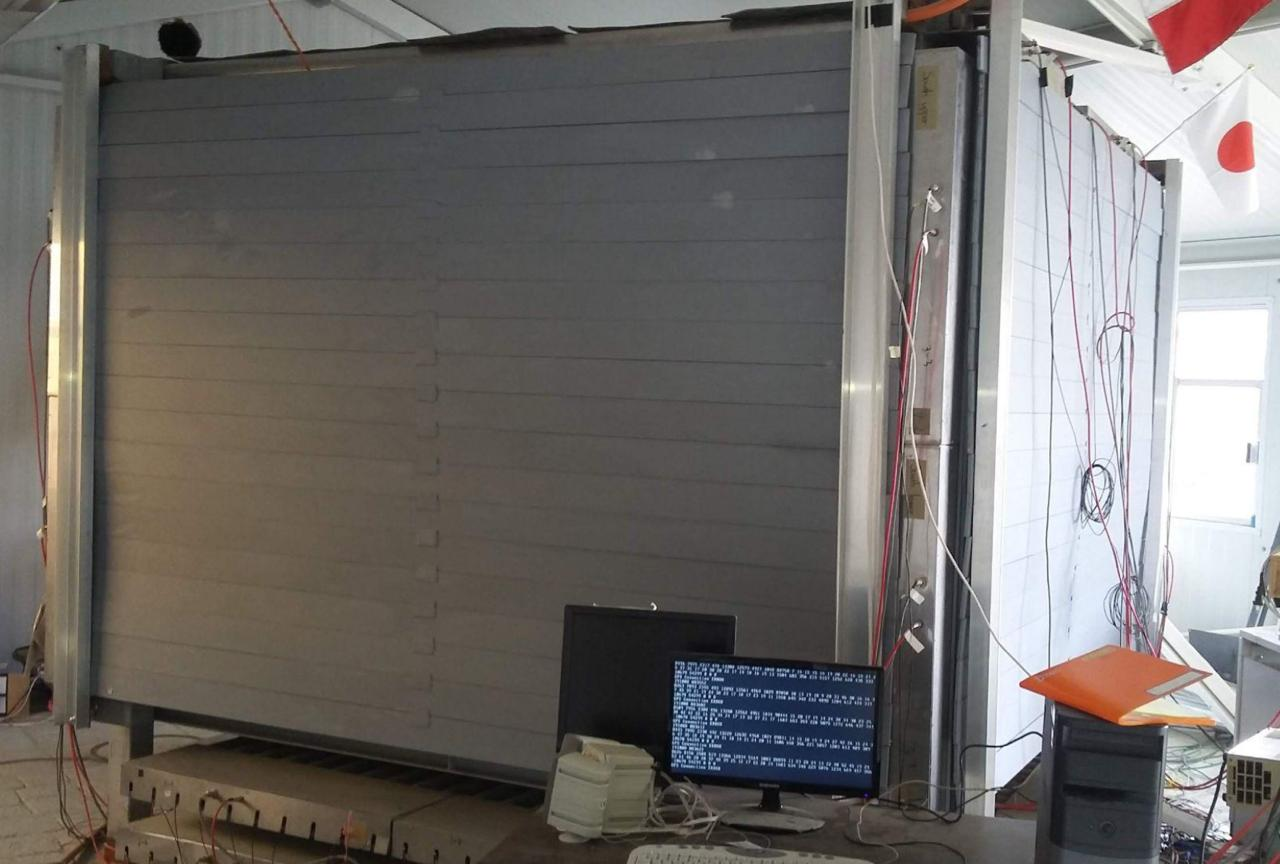
\includegraphics[width=0.61\linewidth]{Figures/tns_new2.jpeg}
                     \end{figure}                     
                \end{itemize}
            \end{column}            
        \end{columns}        

    \end{frame}